\chapter{Resultados}\label{cap:resultados}

Todas las cifras de acierto de este capítulo vienen de las corridas congeladas del 13 de noviembre de 2026, con las
pistas de Demucs de semilla 0. Las gráficas de la comparación con estilos usan la corrida más reciente de cada canción.

\section{Qué detecta la herramienta}\label{sec:res-acierto}

La tabla~\ref{tab:acierto} y la figura~\ref{fig:acierto} comparan la salida de la herramienta con las referencias
corregidas de oído. En promedio, la melodía principal acierta el 49\,\% y la fundamental del acorde, el 85\,\% en los
compases confiables.

\begin{figure}[htbp]
  \centering
  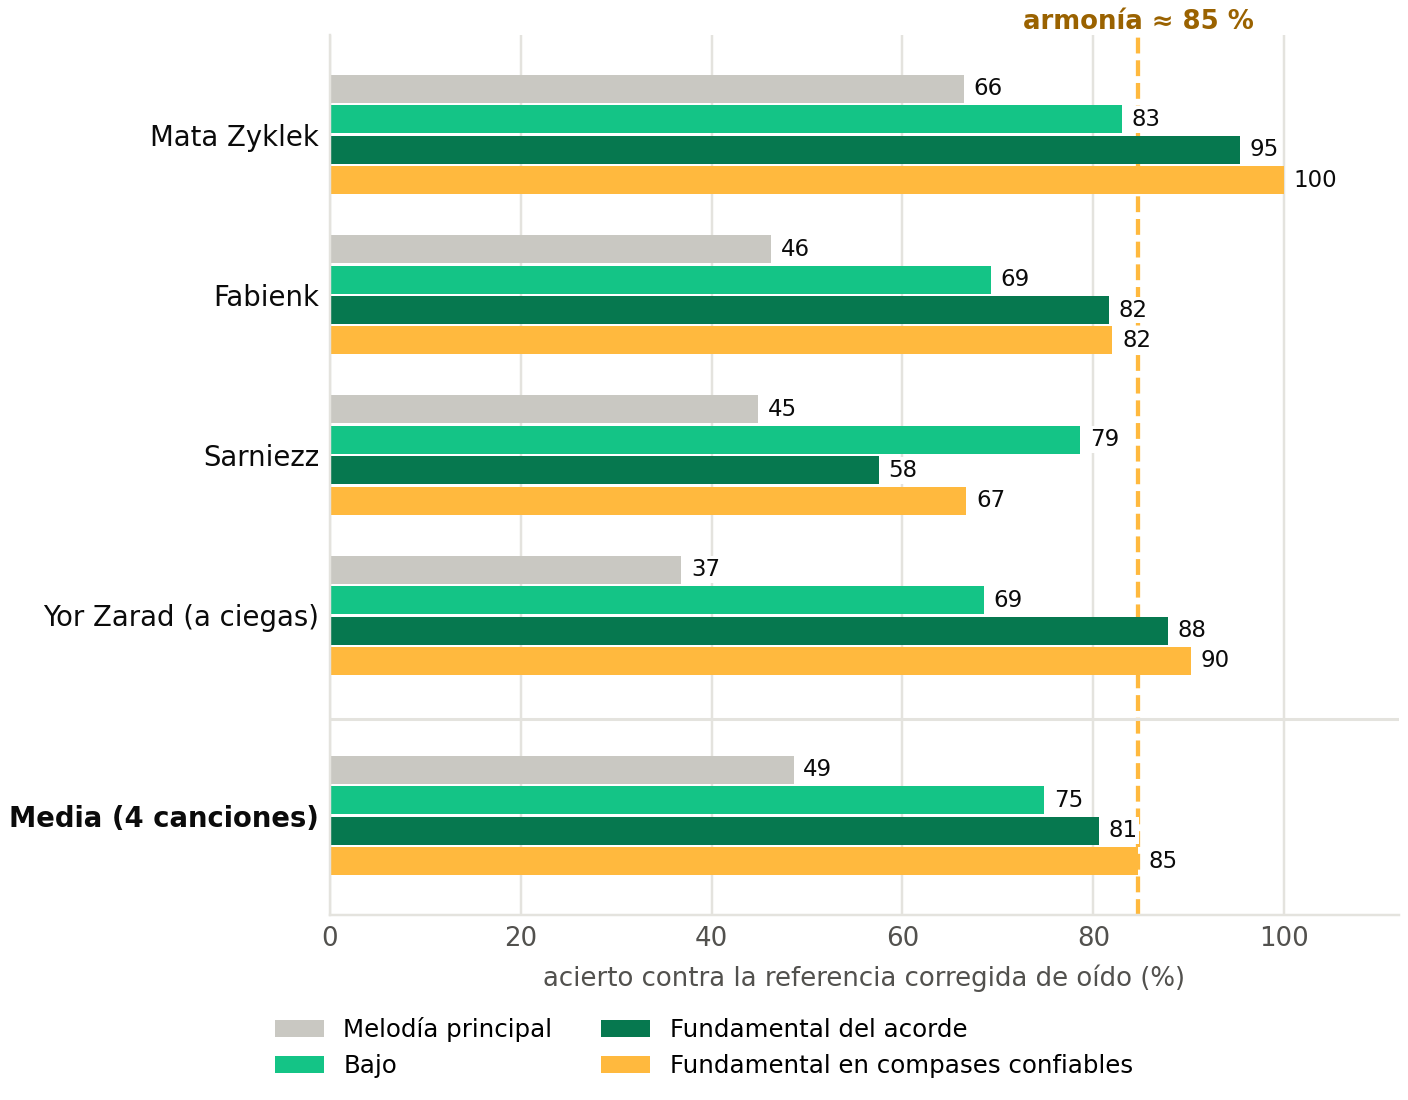
\includegraphics[width=0.72\textwidth]{acierto_herramienta.png}
  \caption{Acierto de la herramienta por canción, contra la referencia corregida de oído. Gris: melodía principal; verde claro: bajo; verde oscuro: fundamental del acorde; amarillo: fundamental en compases confiables, cuya media (línea punteada) es del 85\,\%.}\label{fig:acierto}
\end{figure}

\begin{table}[ht]
  \centering
  \caption{Acierto contra las referencias corregidas de oído (medida F para melodía y bajo; \% del tiempo para la
  fundamental).}\label{tab:acierto}
  \begin{tabular}{@{}lrrrr@{}}
    \toprule
    Canción & Melodía principal & Bajo & Fundamental & Fundamental (confiables) \\
    \midrule
    Mata Zyklek & 66.4 & 83.0 & 95.4 & 100 \\
    Fabienk & 46.2 & 69.2 & 81.6 & 82 \\
    Sarniezz & 44.9 & 78.6 & 57.5 & 67 \\
    Yor Zarad (a ciegas) & 36.8 & 68.6 & 87.8 & 90.2 \\
    \midrule
    \textbf{Media} & \textbf{49} & \textbf{75} & \textbf{81} & \textbf{85} \\
    \bottomrule
  \end{tabular}
\end{table}

\subsection{Por qué la armonía es fiable aunque la melodía no lo sea tanto}

La diferencia entre la melodía y la armonía no es casual. Cuatro rasgos del método la explican:
\begin{enumerate}
  \item \textbf{El bajo manda.} Al decidir la fundamental pesa más el bajo (1 frente a 0.6), que es la voz mejor
  transcrita.
  \item \textbf{Se suma sobre las vueltas del loop.} Un error en una vuelta queda en minoría frente a las demás.
  \item \textbf{La octava no importa.} Una nota una octava arriba es la misma clase de altura. La mayoría de los errores
  de la melodía son la nota correcta en otra octava, o una nota correcta de otro loop de guitarra.
  \item \textbf{Por compás, no por nota.} La melodía exige acertar el ataque a $\pm75$~ms; el acorde solo pide saber qué
  notas suenan en el compás.
\end{enumerate}

Un experimento aparte lo confirma: al cambiar solo el peso de la melodía (tres valores), su acierto varió (Fabienk de
40.8 a 44.2, Sarniezz de 46.0 a 47.9), pero la fundamental quedó idéntica en las tres corridas (82.3 y 72.3). Esas
corridas son de una versión anterior del cuaderno, así que lo que se cita es la invariancia, no los valores absolutos.

\subsection{La prueba ciega}

En Yor Zarad, medida una sola vez sobre la corrida congelada, la melodía principal acierta 36.8 (47.7 sin contar la
octava) y el bajo, 68.6. La armonía sale entre las mejores del álbum: fundamental 87.8\,\% en 99 compases (90.2\,\% en los
confiables), fundamental y calidad 43.0\,\%, bajo 94.2\,\% y el mismo centro (Sol) que la partitura. El fallo principal es
que el riff grave sale una octava arriba, porque la voz aguda nunca baja de Si2; el autor confirmó a ciegas que la
referencia tenía razón.

\subsection{La armonía frente a referencias más completas}

Sumar a la referencia corregida todas las guitarras de Guitar Pro cambia la fundamental en pocos compases (0, 7 y 3\,\%) y
sube el acierto de la herramienta entre 0 y 1.3 puntos (tabla~\ref{tab:ref-completa}): la referencia corregida era
representativa. La partitura de Guitar Pro sola solo es fiable en Mata Zyklek.

\begin{table}[ht]
  \centering
  \caption{Fundamental correcta (\%) según la referencia.}\label{tab:ref-completa}
  \begin{tabular}{@{}lrrr@{}}
    \toprule
    Canción & Corregida & Completa & Guitar Pro sola \\
    \midrule
    Mata Zyklek & 95.4 & 95.4 & 93.8 \\
    Sarniezz & 57.5 & 58.6 & 37.8 \\
    Fabienk & 81.6 & 82.9 & 58.8 \\
    \bottomrule
  \end{tabular}
\end{table}

La función armónica coincide con la de la partitura casi lo mismo que la fundamental (66.0\,\% en Sarniezz, 98.1\,\% en Mata
Zyklek y 82.9\,\% en Fabienk; 90.4, 98.8 y 83.5\,\% en los compases confiables): los errores vienen de la fundamental, no
del etiquetado. Sarniezz es el punto débil: uno de sus acordes más frecuentes, \fl VIIsus2, comparte notas con sus vecinos, y su bajo de
Mi suena un cuarto de tono bajo y la herramienta lo lee como Re\sh+.

\section{Separación: un resultado negativo}\label{sec:res-separacion}

BS-RoFormer separa la guitarra mucho mejor que Demucs según las métricas públicas, pero la melodía de Sarniezz quedó igual
con los dos (tabla~\ref{tab:separacion}). Además, BS-RoFormer tardó 3\,616~s (unos 60 minutos, 13 veces la duración de la
canción) en separarla en CPU.

\begin{table}[ht]
  \centering
  \caption{Demucs frente a BS-RoFormer SW en Sarniezz (\% de acierto contra la partitura corregida).}\label{tab:separacion}
  \begin{tabular}{@{}lrr@{}}
    \toprule
    & Demucs & BS-RoFormer SW \\
    \midrule
    SDR de guitarra (métrica pública, dB) & 5.22 & 9.05 \\
    Melodía principal & 44.9 & 44.9 \\
    Melodía principal, sin octava & 51.1 & 51.8 \\
    Nota más aguda & 35.3 & 30.9 \\
    Bajo & 78.6 & 76.5 \\
    \bottomrule
  \end{tabular}
\end{table}

Por sección, BS-RoFormer ayuda donde suenan dos guitarras con una frase aguda (c.~43--51: de 19.3 a 43.0) y empeora donde
la guitarra toca sola sobre el bajo (c.~27--30: de 55.9 a 40.3). La dificultad está dentro de la guitarra: el looper
superpone varias capas del mismo instrumento y ningún separador las distingue. El resultado no invalida el trabajo:
muestra que la medida no depende del separador y ubica con precisión el cuello de botella, que es separar las capas del
looper, no medir los cuartos de tono. Demucs se mantiene como separador por defecto.

\section{Armonía: fuera de todos los corpus}\label{sec:res-armonia}

Frente a los cuatro corpus de armonía, los estilos más cercanos son el rock y el pop, pero ninguna canción pasa de 17.7
(Utzp en pop), cuando una pieza típica daría 50 (figura~\ref{fig:matriz}). Las canciones con pedal (Mata Zyklek y Utzp)
quedan cerca del borde del rock (12 y 11.7); Fabienk, Sarniezz y Yor Zarad quedan por debajo de 1 en rock. La práctica
común y el jazz no encajan con ninguna canción. La matriz con las 36 canciones medidas, incluidos los repertorios, está en
el apéndice (figura~\ref{fig:g-matriz}).

\begin{figure}[htbp]
  \centering
  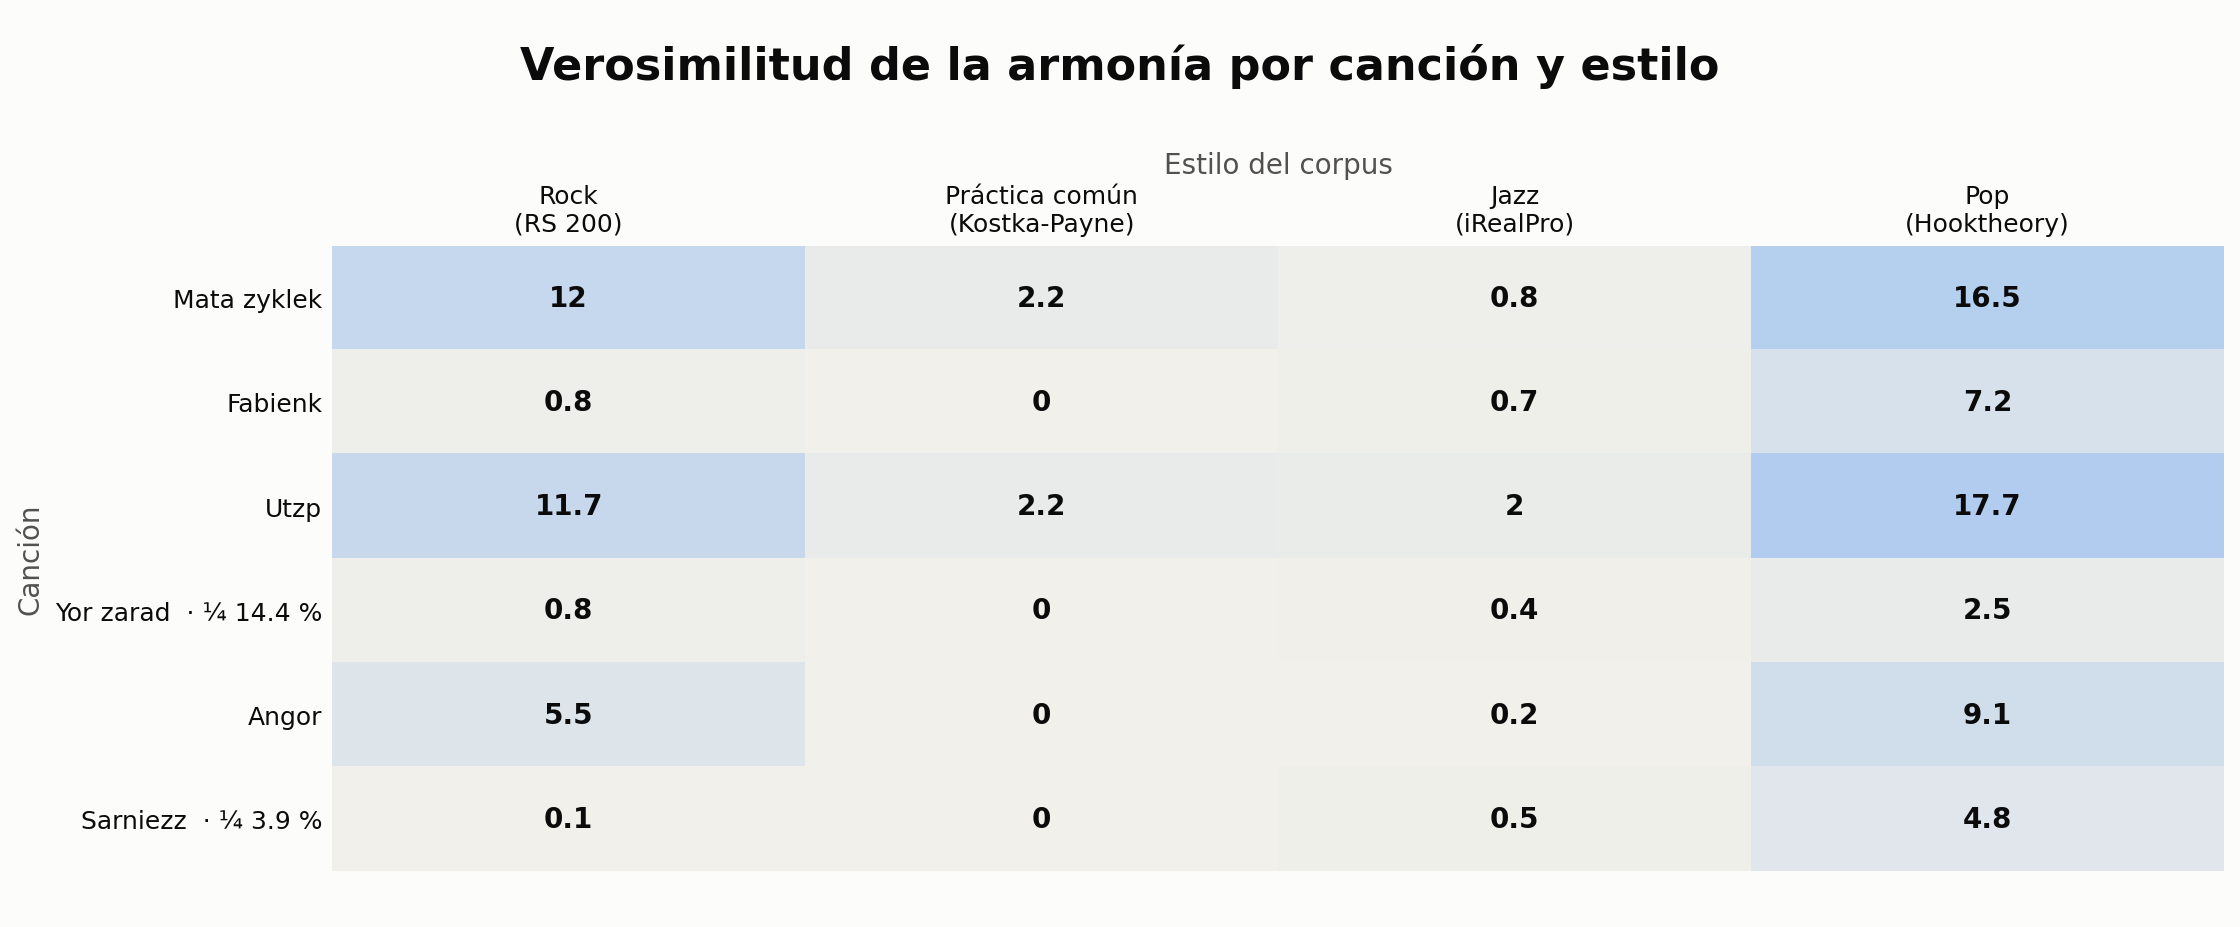
\includegraphics[width=\textwidth]{1a_armonia_matriz_verosimilitud.png}
  \caption{Matriz de verosimilitud armónica del álbum frente a rock (RS~200), práctica común (Kostka-Payne), jazz (iRealPro) y pop (Hooktheory). Percentil: 50 = típica; 0 = más rara que todas. «¼\,\%»: tiempo con fundamental en cuarto de tono.}
  \label{fig:matriz}
\end{figure}

El método no exagera la novedad. Calibrado con 388 piezas reales de rock, comparadas contra las demás, da «estilo
existente» el 92.3\,\% de las veces y «sin vecino» solo el 5.2\,\%. En la banda, el 37.5\,\% de los casos (9 de los 24
bloques de las seis canciones) queda sin vecino.

El mapa de la figura~\ref{fig:mapa} lo muestra de otra forma. Cada canción y cada pieza de corpus se reduce a su reparto
de fundamentales en 12 grados desde su tónica, de modo que la tonalidad no importa, y el análisis de componentes
principales comprime esos doce números en las dos direcciones en que más se diferencian las piezas. El eje horizontal
crece con el peso de II y VI y decrece con el de la tónica; el vertical baja cuando pesan \fl VI, \fl VII y \fl III. Dos
puntos cercanos tienen repartos parecidos. Mata Zyklek y Utzp, que se apoyan en un pedal sobre la tónica, quedan en el
borde del rock; Sarniezz y Fabienk caen donde no hay piezas de ningún corpus, por el peso de \fl VII y \fl III (en
Sarniezz, \fl III ocupa el 42\,\% del tiempo). El mismo mapa con los repertorios de King Gizzard, Zappa, King Crimson y Gentle Giant está en el apéndice
(figura~\ref{fig:g-mapa}). Las estrellas son, de arriba abajo: Mata Zyklek $(-0.48,\ 0.03)$, Angor
$(-0.52,\ -0.05)$, Utzp $(-0.51,\ -0.10)$, Yor Zarad $(-0.46,\ -0.17)$, Fabienk $(-0.21,\ -0.55)$ y Sarniezz
$(-0.21,\ -0.63)$. Angor cae en el mismo punto que «Flying Microtonal Banana» de King Gizzard.

\begin{figure}[htbp]
  \centering
  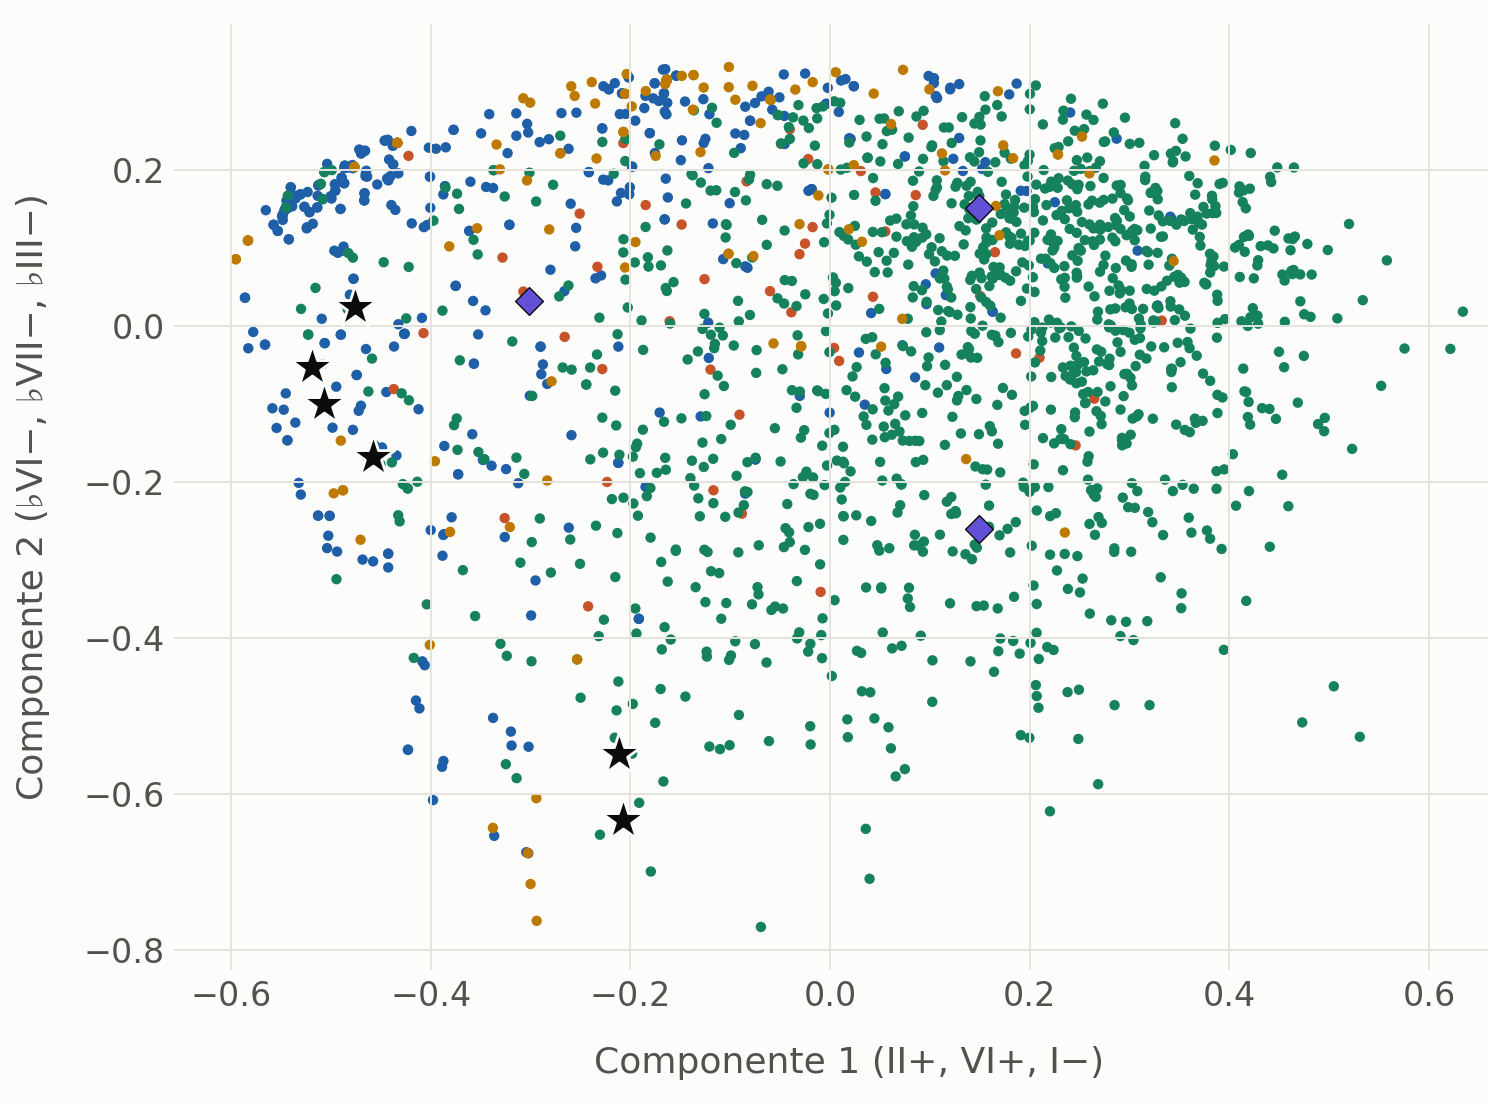
\includegraphics[width=\textwidth]{1b_armonia_mapa_fundamentales.png}
  \caption{Mapa de fundamentales. Puntos del fondo: rock (azul, RS~200, 400 piezas), práctica común (rojo, Kostka-Payne, 46), jazz (verde, iRealPro, 1186) y pop (naranja, Hooktheory, 121). Estrellas: la banda; rombos: Primus. Puntos cercanos tienen repartos de fundamentales parecidos; los ejes son componentes principales (entre paréntesis, los grados que más pesan).}\label{fig:mapa}
\end{figure}

Frente al pop de Hooktheory, la banda queda a una distancia de Jensen-Shannon de 0.40 a 0.59, cuando los nueve álbumes de
pop entre sí no pasan de 0.07. Los ejes de Lendvai muestran rasgos que el círculo de quintas no ve: en Sarniezz, el 24\,\%
de los cambios de la partitura queda dentro del eje de tónica (I $\leftrightarrow$ \fl III, Mi $\leftrightarrow$ Sol), una
sustitución y no un movimiento por quintas; las canciones con cuartos de tono se mueven entre un eje de Lendvai y uno
neutro (Mata Zyklek D $\leftrightarrow$ D--S, Yor Zarad T $\leftrightarrow$ D--S).

La tabla~\ref{tab:funciones} resume el movimiento armónico de cada canción. Tres patrones se distinguen: los pedales
(Mata Zyklek, Utzp y Angor), casi sin cambios de fundamental y con más del 90\,\% del tiempo en función de tónica; el
vaivén modal de Fabienk y Sarniezz, con decenas de cambios y alrededor de un tercio del tiempo en dominante modal
(\fl VII, sin sensible); y el vaivén microtonal de Yor Zarad, cuyos cambios son todos entre I y \fl II+, fuera de la tabla
de progresiones de Piston.

\begin{table}[ht]
  \centering\small
  \caption{Funciones y progresiones (compases confiables). T, D, N: porcentaje del tiempo en función de tónica,
  dominante y neutra.}\label{tab:funciones}
  \begin{tabular}{@{}lrrrrrl@{}}
    \toprule
    Canción & Cambios & Por quintas & T & D & N & Progresión más frecuente \\
    \midrule
    Mata Zyklek & 2 & 100\,\% & 92.7 & 7.3 & 0 & I5 $\to$ Vsus4 $\to$ I \\
    Fabienk & 86 & 51\,\% & 63.1 & 36.9 & 0 & \fl VII $\to$ \fl III \\
    Sarniezz & 56 & 59\,\% & 66.6 & 29.5 & 3.9 & \fl III $\leftrightarrow$ \fl VIIsus2 \\
    Yor Zarad & 11 & 0\,\% & 85.6 & 0 & 14.4 & I5 $\leftrightarrow$ \fl II+5 \\
    Utzp & 9 & 22\,\% & 97.7 & 2.3 & 0 & \fl VIIsus2 $\to$ Iaum \\
    Angor & 0 & — & 100 & 0 & 0 & — \\
    \bottomrule
  \end{tabular}
\end{table}

\section{Melodía: cuartos de tono como grados fijos}\label{sec:res-melodia}

La tabla~\ref{tab:cuartos} y la figura~\ref{fig:uso} muestran cómo usa cada canción los cuartos de tono.

\begin{figure}[htbp]
  \centering
  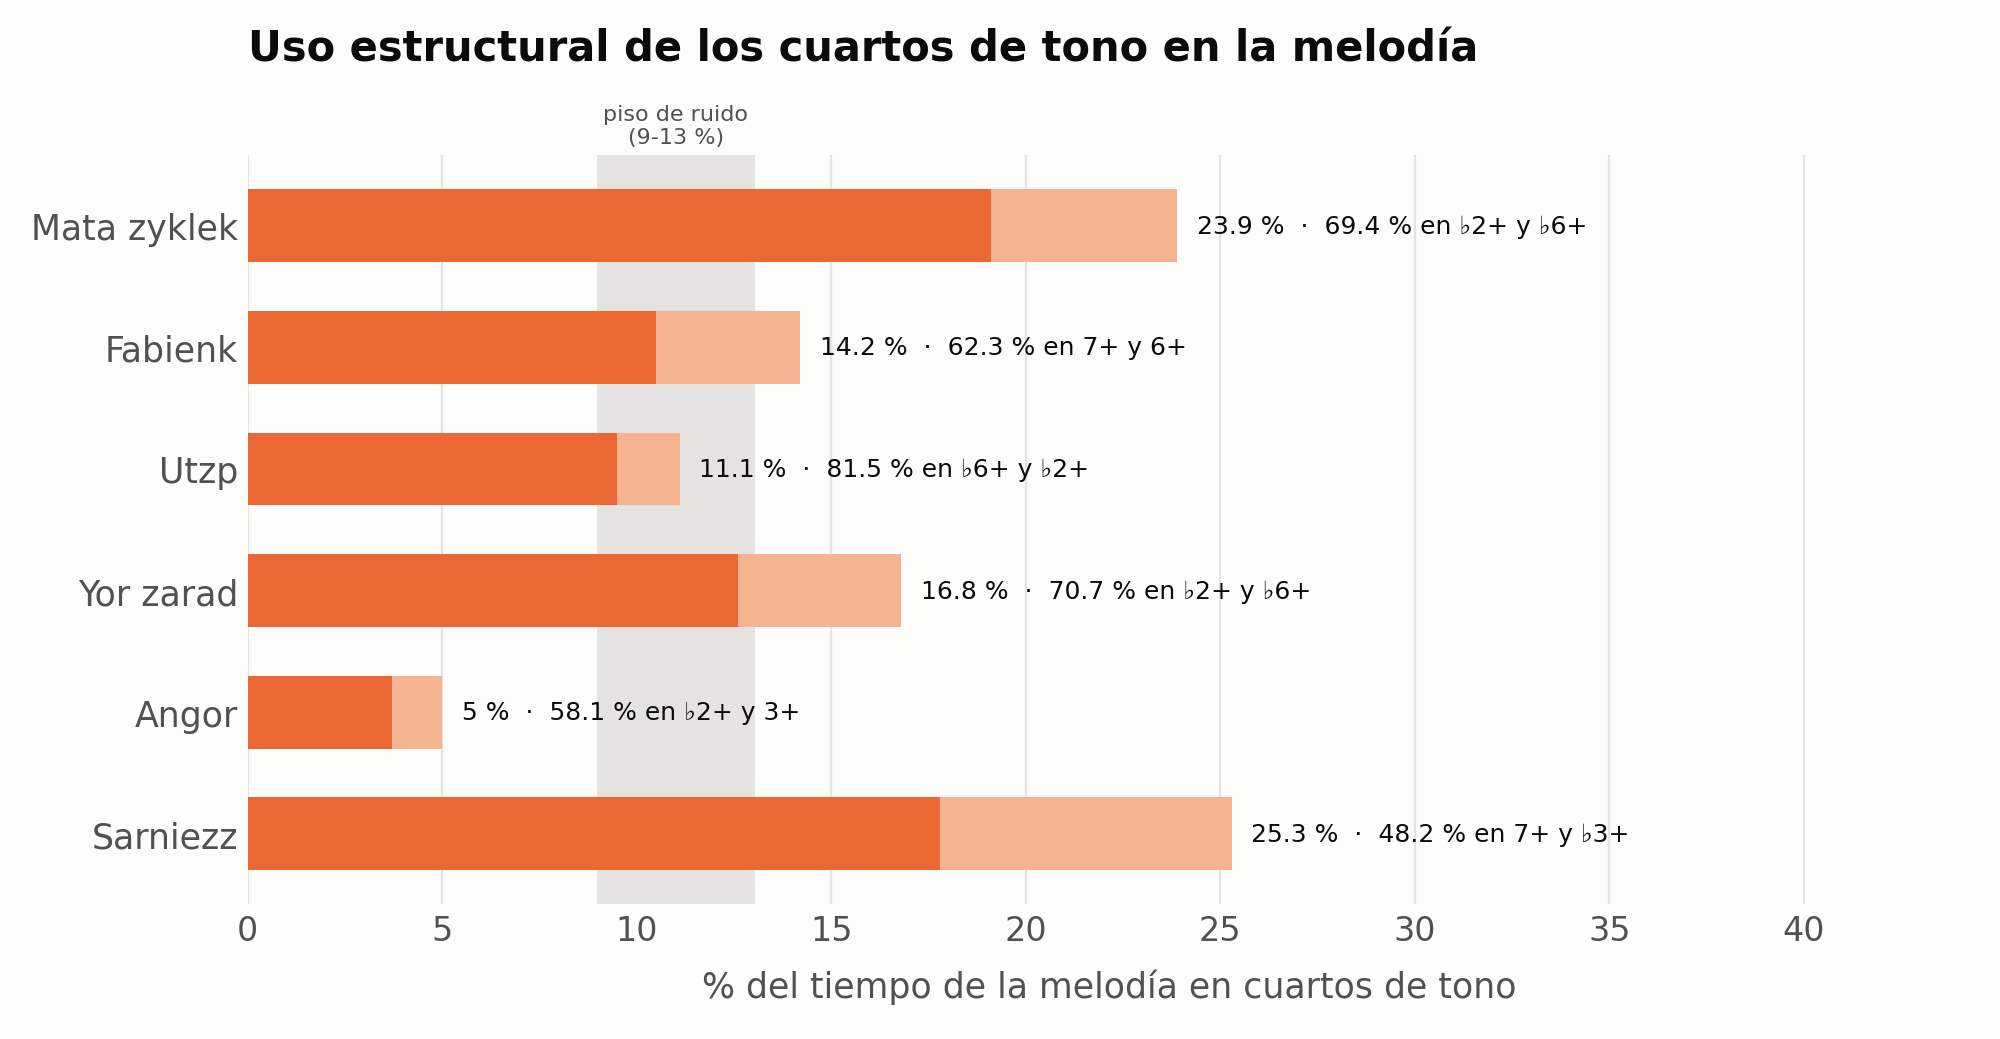
\includegraphics[width=0.9\textwidth]{2a_melodia_uso_cuartos_de_tono.png}
  \caption{Cuartos de tono en la melodía (\% del tiempo). Oscuro: como grado sostenido; claro: como adorno. Franja gris: piso de ruido medido en Primus (9--13\,\%). A la derecha de cada barra, la fracción que cae en los dos grados más usados.}\label{fig:uso}
\end{figure}

\begin{table}[ht]
  \centering
  \caption{Uso de los cuartos de tono en la melodía (\% del tiempo de la voz aguda).}\label{tab:cuartos}
  \begin{tabular}{@{}lcrrrr@{}}
    \toprule
    Canción & Centro & \shortstack{En \cuarto{}\\de tono} & \shortstack{Como\\grado} & \shortstack{Como\\inflexión} & \shortstack{En los dos grados\\más usados} \\
    \midrule
    Mata Zyklek & Sol & 23.9 & 19.1 & 4.8 & 69.4 \\
    Fabienk & Mi & 14.2 & 10.5 & 3.7 & 62.3 \\
    Utzp & Mi & 11.1 & 9.5 & 1.6 & 81.5 \\
    Yor Zarad & Sol & 16.8 & 12.6 & 4.2 & 70.7 \\
    Angor & Sol & 5.0 & 3.7 & 1.3 & 58.1 \\
    Sarniezz & Mi & 25.3 & 17.8 & 7.5 & 48.2 \\
    \midrule
    Primus (control) & & 9--13 & & & 28--37 \\
    \bottomrule
  \end{tabular}
\end{table}

Entre el 48 y el 82\,\% de los cuartos de tono de cada canción caen en solo dos grados, que vuelven en cada vuelta del
loop; en Primus están repartidos (28--37\,\%). Son grados de la escala, no adornos: la mayor parte del tiempo en cuarto de
tono es como grado sostenido. Angor, con 5\,\%, queda por debajo del piso de ruido y no cuenta. Las mismas barras para
las 36 canciones y la escala de cada una están en el apéndice (figuras~\ref{fig:g-uso} a~\ref{fig:g-escalas2}).

El círculo de 24-EDO (figura~\ref{fig:circulo}) muestra qué escalas forman esos grados. Aparecen dos familias:
\begin{itemize}
  \item \textbf{Frigia:} \fl2+ y \fl6+ sobre un frigio (Mata Zyklek, Yor Zarad y Utzp).
  \item \textbf{Dórica:} 7+, 6+ y \fl3+ sobre un dórico (Sarniezz: 7+ y \fl3+; Fabienk: 7+ y 6+).
\end{itemize}

\begin{figure}[htbp]
  \centering
  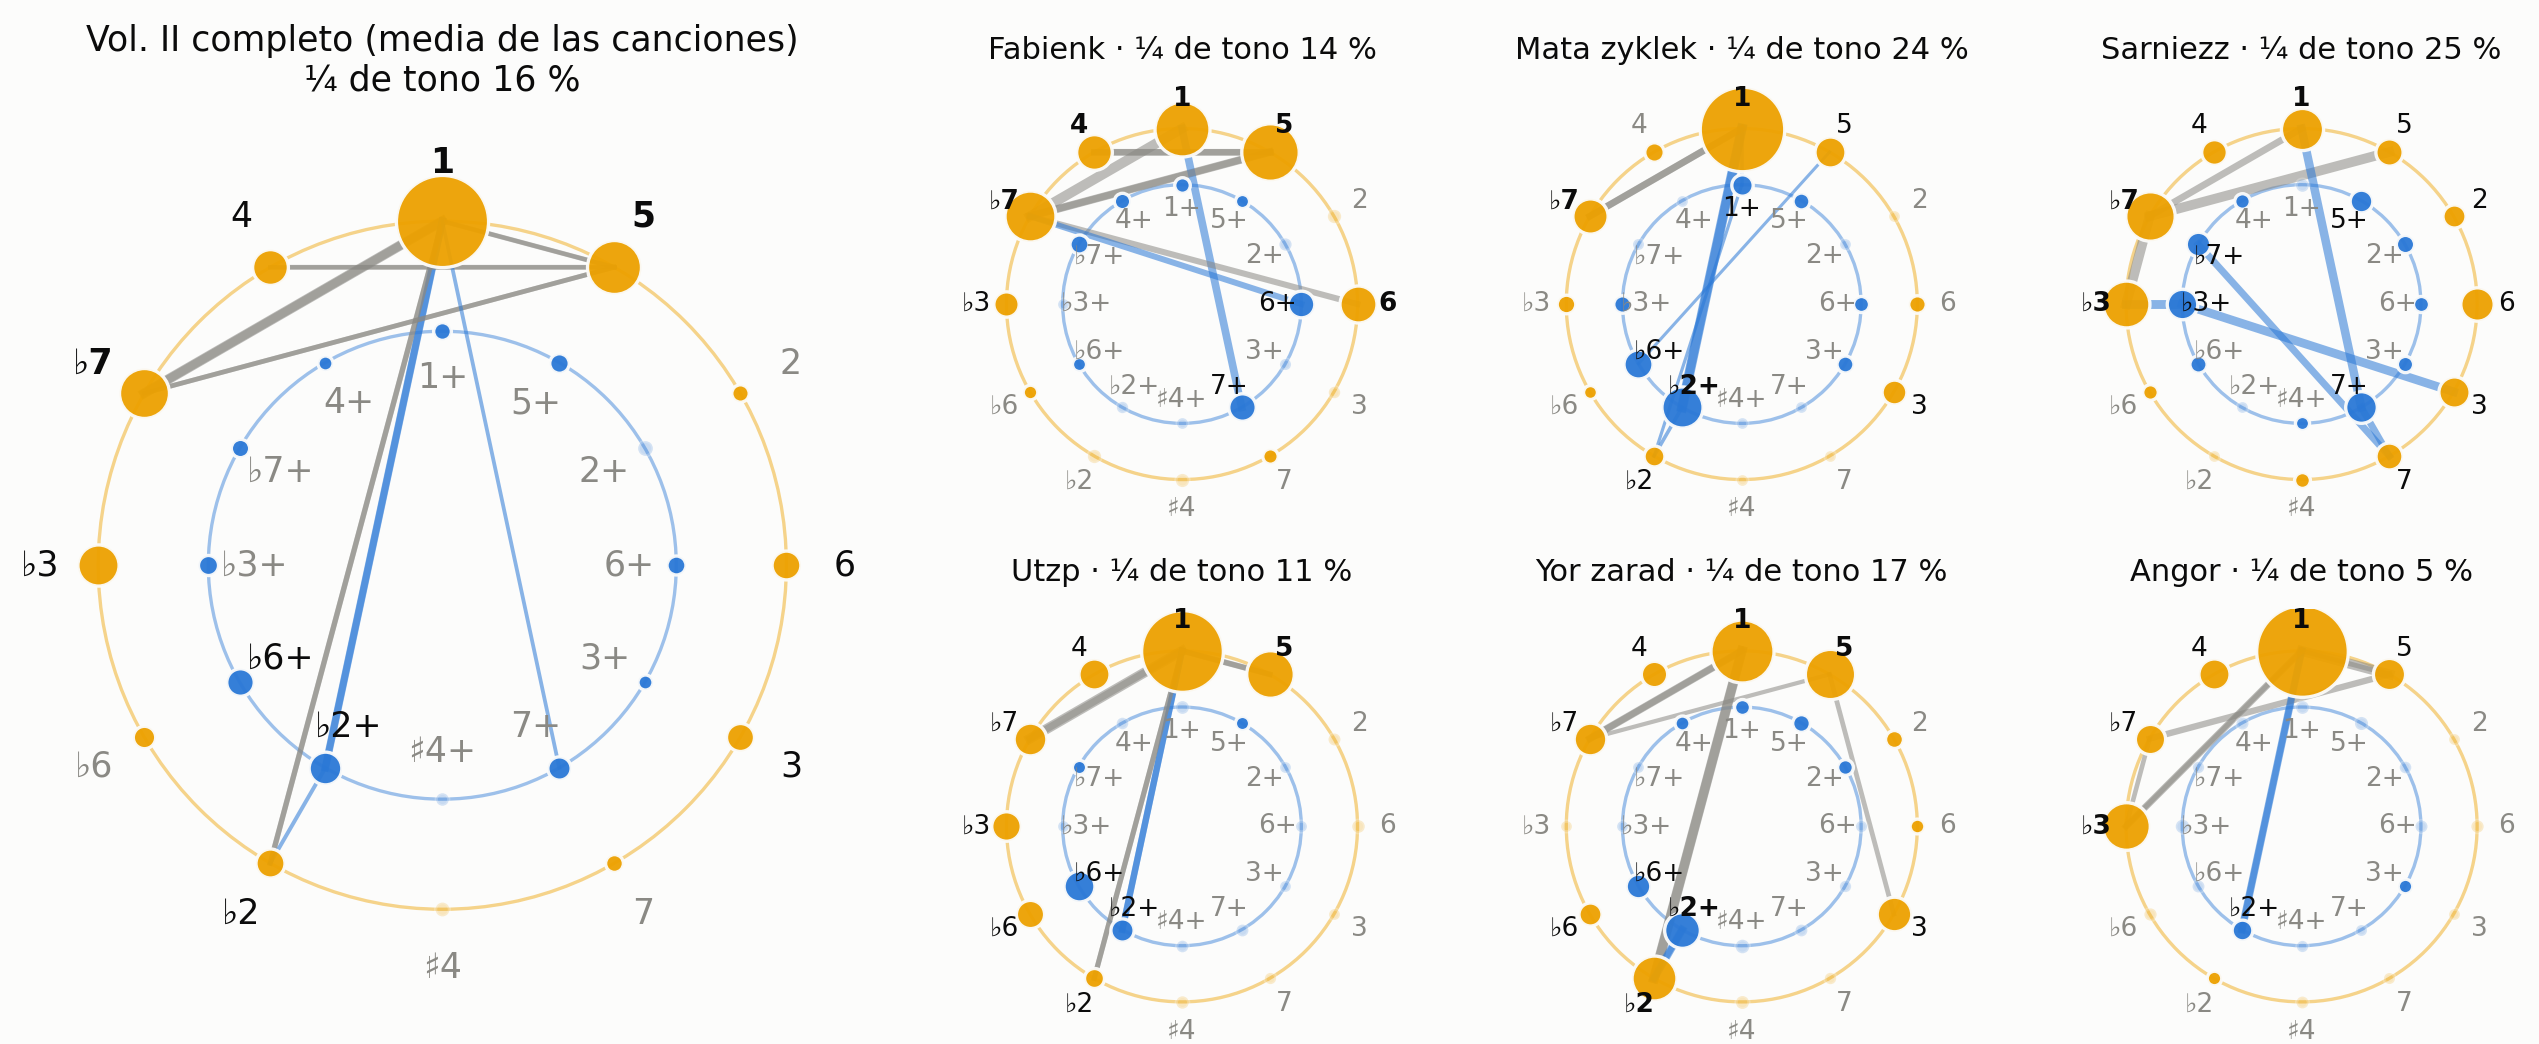
\includegraphics[width=\textwidth]{2b_melodia_circulo_24edo.png}
  \caption{Círculo de quintas en 24-EDO: el álbum (izquierda) y cada canción. Anillo amarillo: campo regular; anillo azul: campo de cuarto de tono. Área del punto: tiempo melódico en el grado; líneas grises: pasos dentro de un campo; azules: pasos entre campos.}\label{fig:circulo}
\end{figure}

La tabla~\ref{tab:familias} compara esas familias con los corpus. La frigia no es exclusiva de la banda: es el par más
común del radif persa y el de King Gizzard. Lo que ningún corpus medido tiene es la familia dórica. El corpus indostánico
no aporta cuartos de tono, porque sus 22 \emph{shrutis} caen todos en grados regulares al pasarlos a 24-EDO.

\begin{table}[ht]
  \centering\small
  \caption{Los dos grados en cuarto de tono más usados de cada pieza, por corpus.}\label{tab:familias}
  \begin{tabular}{@{}lrrr@{}}
    \toprule
    & \shortstack{Con cuartos\\de tono ($\ge 2$\,\%)} & \shortstack{Familia frigia\\(\fl2+, \fl6+)} & \shortstack{Familia dórica\\(7+, 6+, \fl3+)} \\
    \midrule
    Radif Corpus & 190 de 229 & 43 & 0 \\
    Indostánico & 0 de 50 & — & — \\
    King Gizzard (medido) & 9 de 9 & 5 & 0 \\
    Angine de Poitrine & 6 de 6 & 3 & 2 \\
    \bottomrule
  \end{tabular}
\end{table}

\subsection{El círculo en movimiento}\label{sec:circulo-vivo}

Para la presentación se exportó un fragmento de Mata Zyklek (de 0:42 a 1:12) que anima las notas sobre el círculo,
sincronizadas con el audio. Con tónica Sol, las voces giran sobre Sol y Sol\sh+ (\fl2+), el cuarto de tono del riff.
Frente a la referencia corregida de oído, la herramienta da el mismo grado el 90\,\% del tiempo en la voz aguda y el
88\,\% en la grave, y cuando falla lee Sol\sh+ como Sol: se queda corta, no inventa cuartos de tono.

La exportación exigió dos correcciones. Las notas iban adelantadas, porque la ventana centrada de 4096 muestras ya «ve» la
nota cuando empieza a cubrirla; el mejor acuerdo con pYIN se obtuvo atrasándolas 60~ms en la voz aguda y 55~ms en la
grave, sin deriva a lo largo de la canción. Y se quitaron las notas de menos de 0.15~s de grados que suman menos del 2\,\%
del tiempo de la voz: tres notas de Do que eran errores de quinta (Do es el tercer armónico de Fa).

\section{Desplazamiento de campos}\label{sec:res-haba}

Levi McClain y David Bennett sostienen que la banda usa los cuartos de tono de forma «horizontal», en la melodía, y casi
nunca «vertical», en los acordes, como proponía Hába \citep{mcclain2026,bennett2026}. Para ponerlo a prueba se midió la
\emph{mezcla vertical} $V$: en una rejilla de 20~ms, la fracción del tiempo en que suenan a la vez la voz aguda y el bajo
y están en campos distintos (sección~\ref{sec:campos}). El modelo nulo desplaza el bajo en bloque un tiempo al azar (al
menos 2~s, de forma circular), lo que conserva cuántos cuartos de tono tiene cada voz y su ritmo, pero rompe su
coordinación; $p$ es la fracción de desplazamientos con una mezcla igual o menor que la observada.

\begin{table}[ht]
  \centering
  \caption{Mezcla vertical de campos: observada frente a la esperada por azar.}\label{tab:haba}
  \begin{tabular}{@{}llrrr@{}}
    \toprule
    Grupo & Canción & Observada & Azar & $p$ \\
    \midrule
    Banda & Sarniezz & 15.4\,\% & 38.5\,\% & $< 0.002$ \\
    & Mata Zyklek & 12.7\,\% & 35.8\,\% & $< 0.002$ \\
    & Fabienk & 12.7\,\% & 25.2\,\% & $< 0.002$ \\
    & Yor Zarad & 17.8\,\% & 33.0\,\% & $< 0.002$ \\
    & Utzp & 11.4\,\% & 20.3\,\% & $< 0.002$ \\
    & Angor & 4.7\,\% & 8.0\,\% & 0.006 \\
    \midrule
    Primus & Tommy the Cat & 19.6\,\% & 22.7\,\% & 0.006 \\
    & My Name Is Mud & 20.8\,\% & 21.8\,\% & 0.218 \\
    & Jerry Was a Race Car Driver & 18.2\,\% & 20.6\,\% & $< 0.002$ \\
    \midrule
    King Gizzard & Flying Microtonal Banana & 5.8\,\% & 11.6\,\% & $< 0.002$ \\
    & Doom City & 24.5\,\% & 33.7\,\% & 0.020 \\
    & Melting & 16.9\,\% & 26.5\,\% & 0.002 \\
    \bottomrule
  \end{tabular}
\end{table}

En la banda, la mezcla observada es entre un 35 y un 60\,\% de la esperada por azar; en Primus, entre un 86 y un 95\,\%
(tabla~\ref{tab:haba}). Es decir, cuando la guitarra está en un cuarto de tono, el bajo tiende a acompañarla en el mismo
campo, o a callar, mucho más de lo que daría la casualidad: la banda evita mezclar campos en vertical, como Hába. En
Primus, donde todo cuarto de tono es error de medición, la mezcla queda cerca del azar. En Mata Zyklek y Fabienk, además,
los cuartos de tono caen en el pulso menos que las notas regulares (16 frente a 29\,\%, y 15 frente a 34\,\%; $p < 0.002$
en ambos), lo que es coherente con un uso melódico.

El círculo de la figura~\ref{fig:circulo} ya separaba los dos campos: el anillo amarillo es el campo regular y el azul,
el de cuarto de tono, y la mayoría de los pasos melódicos frecuentes quedan dentro de un mismo campo. La
figura~\ref{fig:campos-tiempo} añade el tiempo: los cuartos de tono no se reparten de forma pareja, sino que se agrupan en
tramos de cada canción, y la mezcla de campos entre guitarra y bajo aparece en muchos compases, pero baja: casi siempre ocupa una parte
pequeña del compás, con pocos picos. La
figura~\ref{fig:campos-resumen} compara las tres pruebas (mezcla evitada, pasos de cuarto de tono entre las notas que ya
tocan uno y presencia en el pulso) en la banda, los repertorios comparados y Primus. En la primera, las seis canciones de
la banda evitan la mezcla entre un 40 y un 65\,\%, lejos del rango del control; los repertorios se reparten a ambos lados,
y algunos llegan al nivel de la banda: «Open Water» y «Flying Microtonal Banana» de King Gizzard, «The Black Page \#1»
de Zappa y «The Runaway» de Gentle Giant. En la figura, un punto vacío indica $p \geq 0.003$, el umbral corregido por
Bonferroni para unas 18 canciones; por eso Angor y «Tommy the Cat» ($p = 0.006$ en la tabla~\ref{tab:haba}) aparecen
como no significativos.

Los acordes dan otra forma de ver la separación, porque una tríada con tercera neutra mezcla campos por construcción
(proposición~\ref{prop:neutra}). En los compases confiables, la herramienta lee la calidad «n» en 2 de los 658 compases de
la banda (0.3\,\%), uno en Utzp y uno en Sarniezz, y en 1 de los 196 de Primus (0.5\,\%), que es el piso de error. King
Gizzard la usa más: 42 de 1120 compases (3.8\,\%), sobre todo en «Melting» (20 de 110), «Nuclear Fusion» (11 de 124) y
«Billabong Valley» (7 de 113). Zappa, King Crimson y Gentle Giant quedan entre el 0.6 y el 1.7\,\%. La banda no arma
acordes con tercera neutra, lo que es coherente con un uso melódico de los cuartos de tono.

\begin{figure}[htbp]
  \centering
  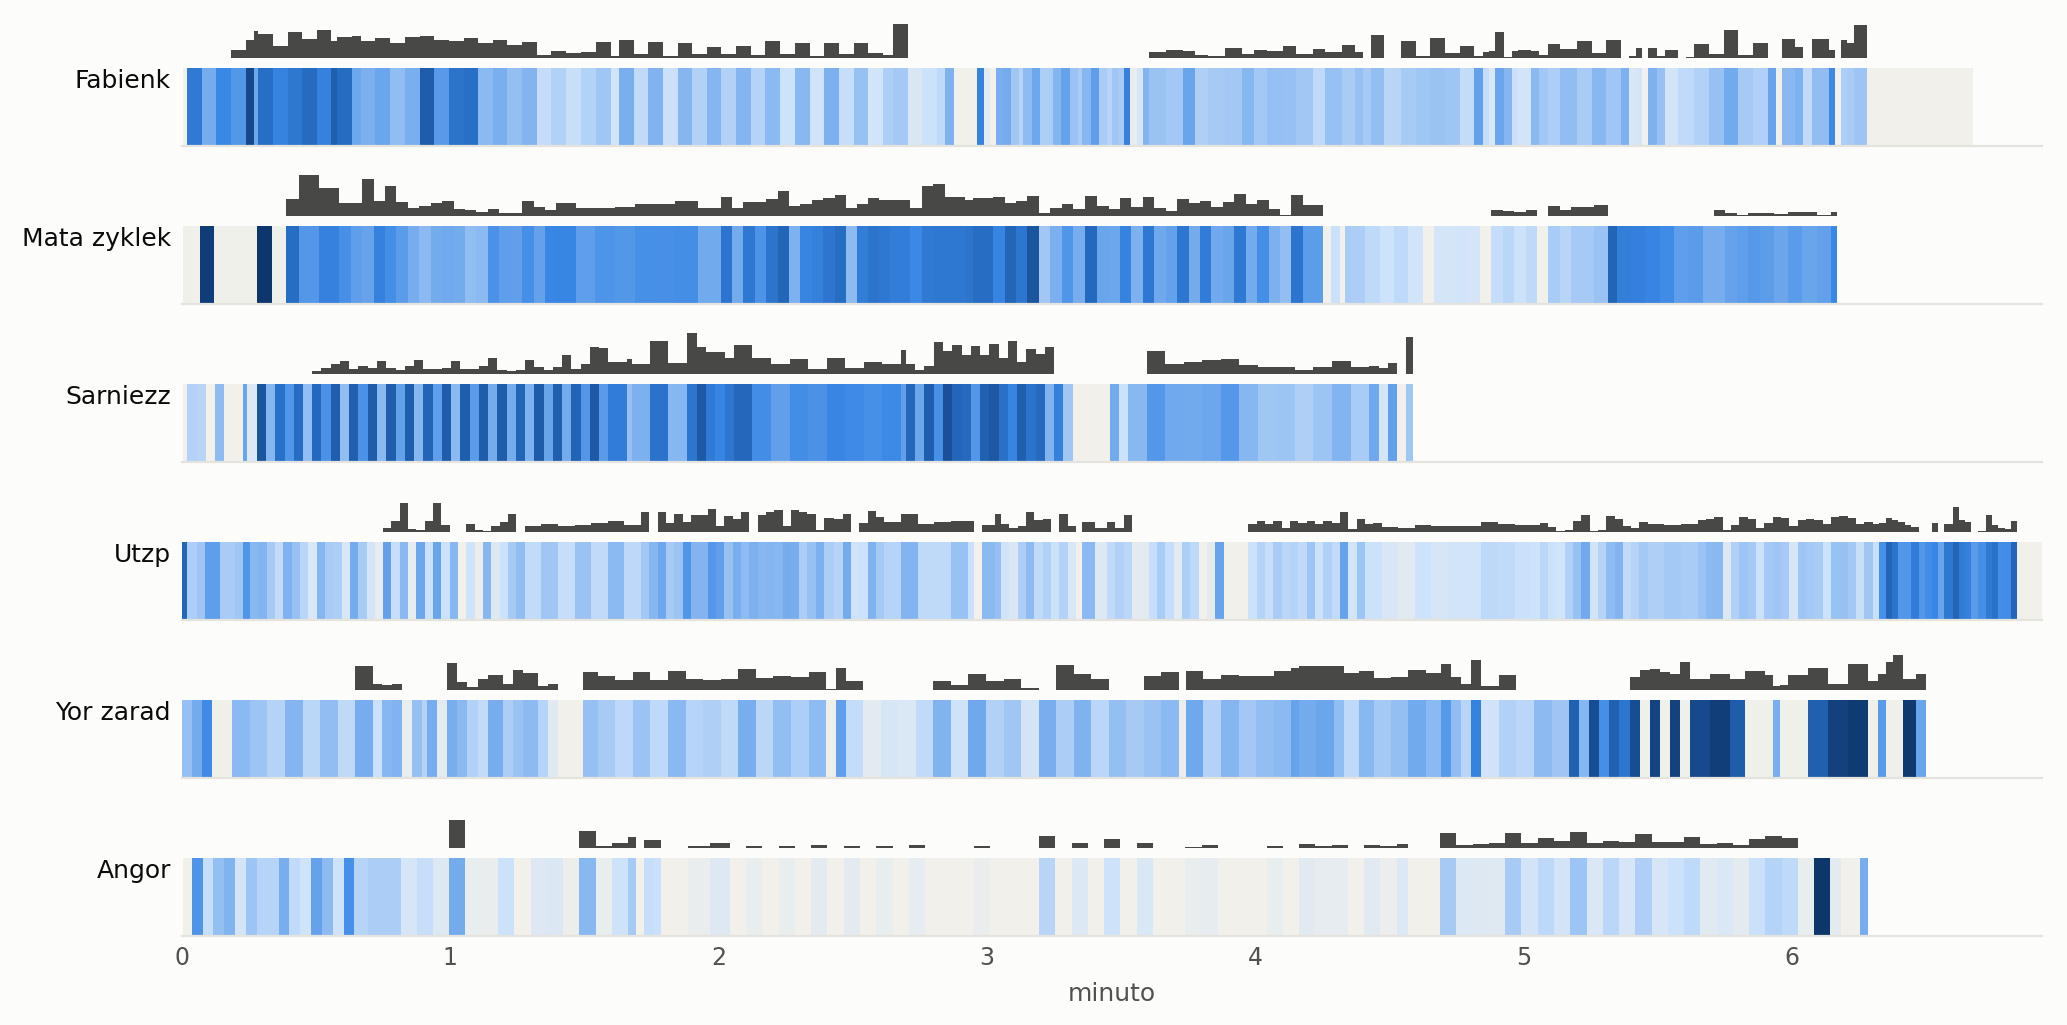
\includegraphics[width=\textwidth]{g_campos_tiempo.png}
  \caption{Cuartos de tono a lo largo de cada canción (eje en minutos). Franja: porcentaje de cada compás en cuarto de tono, de blanco (0\,\%) a azul oscuro (60\,\%). Barras negras: compases con guitarra y bajo en campos distintos (alto completo = 50\,\% o más).}\label{fig:campos-tiempo}
\end{figure}

\begin{figure}[htbp]
  \centering
  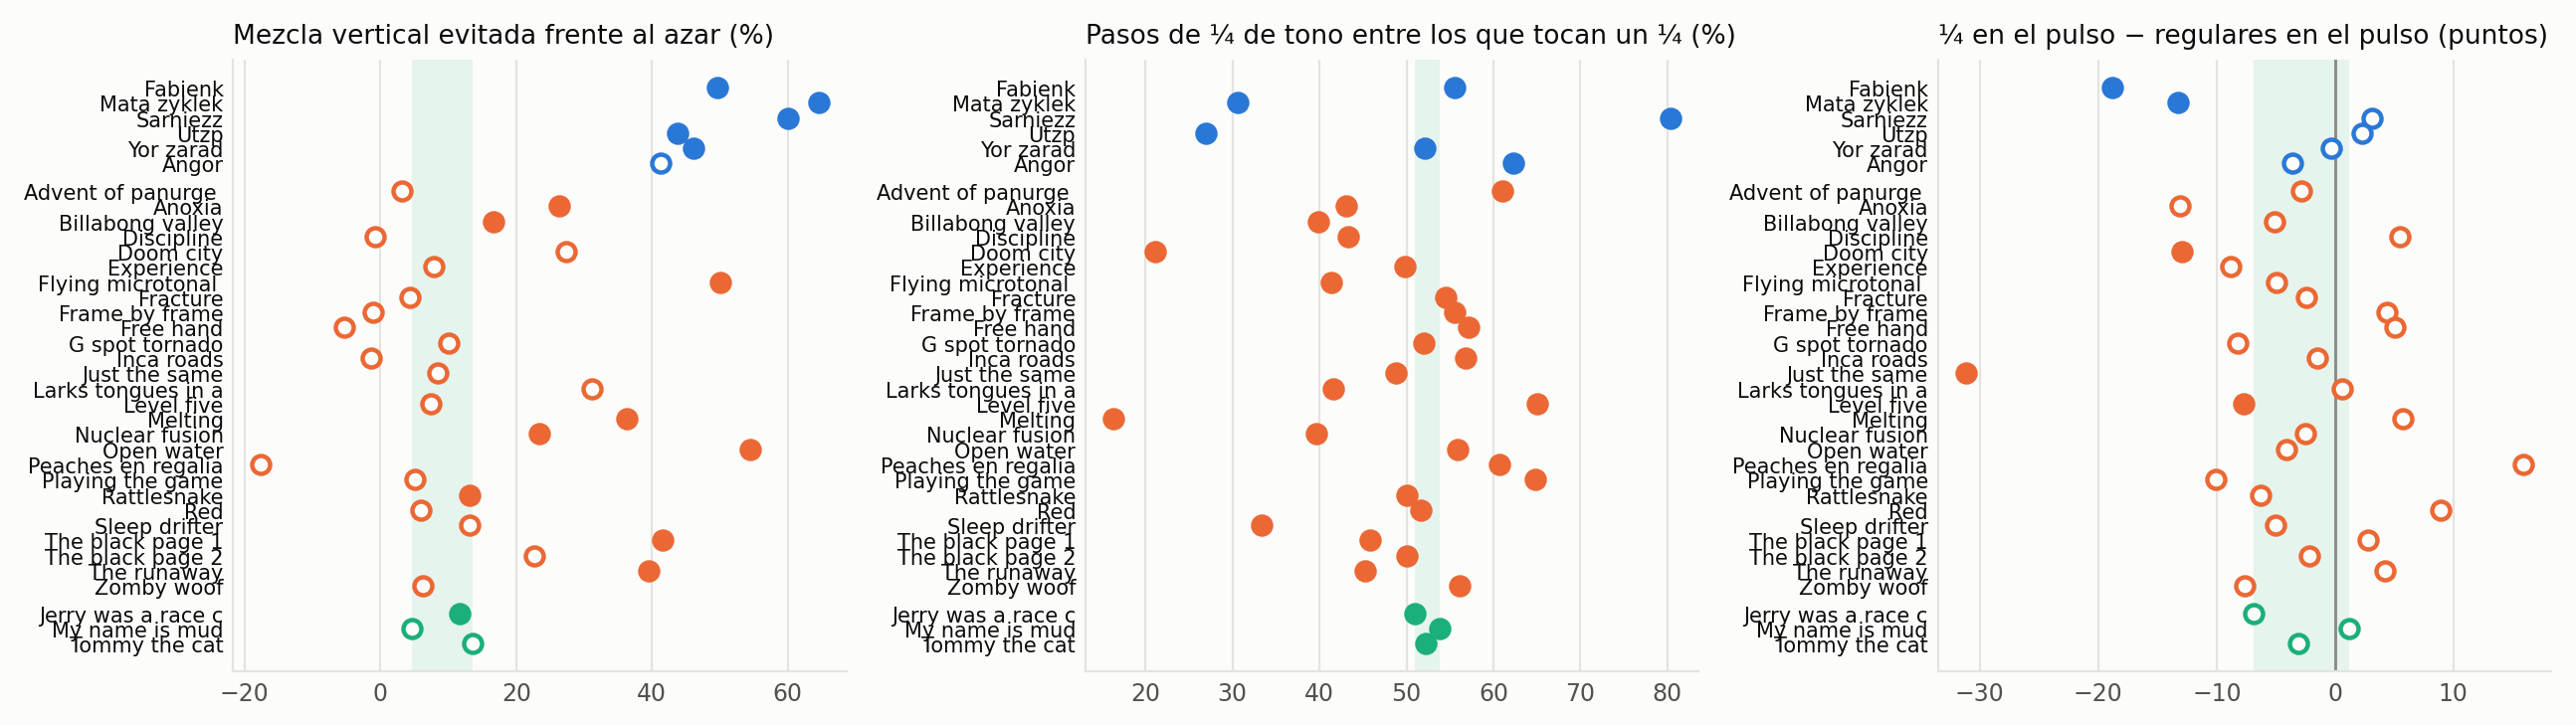
\includegraphics[width=\textwidth]{g_campos_resumen.png}
  \caption{Tres pruebas de separación de campos, una canción por fila. Izquierda: mezcla vertical evitada frente al azar (\%); centro: pasos de cuarto de tono entre las notas que ya están en cuarto de tono (\%); derecha: diferencia entre los cuartos de tono y las notas regulares que caen en el pulso (puntos). Azul: la banda; naranja: repertorios comparados (King Gizzard, Zappa, King Crimson y Gentle Giant); verde: Primus. Círculo vacío: no significativo ($p \ge 0.003$); franja verde: rango del control.}\label{fig:campos-resumen}
\end{figure}

\section{Metro: ciclos de 5 y de 7}\label{sec:res-metro}

\begin{table}[ht]
  \centering
  \caption{Mejor periodo de repetición $R(\ell)$ de cada canción.}\label{tab:ciclos}
  \begin{tabular}{@{}lrrr@{}}
    \toprule
    Canción & Tempo (BPM) & Mejor periodo (corcheas) & $R$ \\
    \midrule
    Mata Zyklek & 94 & 20 (dos compases de 5/4) & 0.82 \\
    Fabienk & 129 & 28 (dos compases de 7/4) & 0.87 \\
    Yor Zarad & 108 & 28 & 0.80 \\
    Angor & 99 & 24 & 0.83 \\
    Sarniezz & 115 & 32 & 0.83 \\
    Utzp & 129 & 32 & 0.87 \\
    \midrule
    Tommy the Cat (Primus) & 129 & 8 & 0.44 \\
    Jerry Was a Race Car Driver (Primus) & 123 & 8 & 0.45 \\
    \bottomrule
  \end{tabular}
\end{table}

El riff de Mata Zyklek se repite cada 20 corcheas: dos compases de 10 corcheas, es decir, de 5/4. El de Fabienk, cada 28:
dos compases de 7/4 (tabla~\ref{tab:ciclos} y figura~\ref{fig:ciclos}). Son los compases que menciona la banda y los que
planteaba la hipótesis. Sarniezz y Utzp, en cambio, van en 4, con picos en 32 corcheas. Los ciclos de la banda son mucho
más estables que los de Primus ($R \approx 0.8$ frente a 0.44). Varias canciones mezclan compases dentro de la misma
pieza: Fabienk pasa el 53\,\% del tiempo en compases de 7, el 18\,\% en 4 y el 9\,\% en 3. El periodo de 28 corcheas de
Yor Zarad es, como en Fabienk, un par de compases de 7/4: el 7 domina el centro de la canción y el 4 aparece al principio
y al final. El de 24 corcheas de Angor es un par de compases de 6/4, el compás de 83 de sus 113 compases; Angor no
tiene referencia de oído, así que esta lectura no está contrastada.

\begin{figure}[htbp]
  \centering
  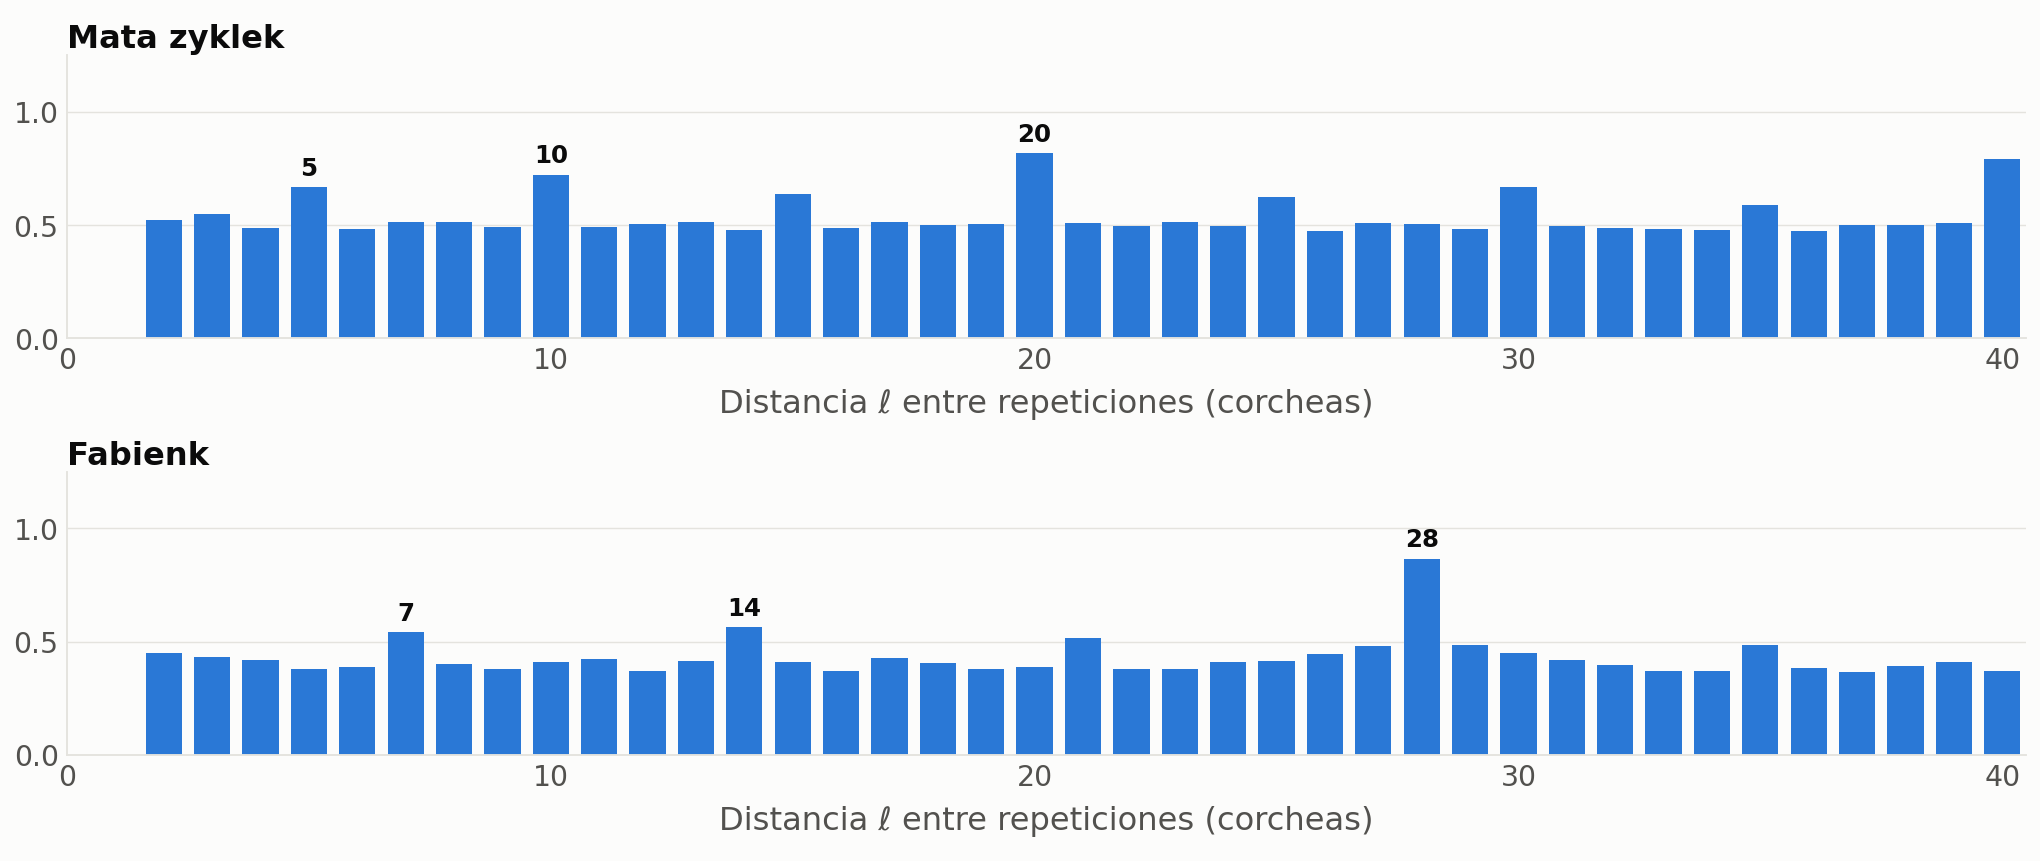
\includegraphics[width=0.75\textwidth]{3a_sintesis_ciclos_metricos.png}
  \caption{Repetición $R(\ell)$ en Mata Zyklek y Fabienk según la distancia $\ell$ en corcheas. Un pico alto y aislado es un ciclo largo y estable: 20 y 28 corcheas.}
  \label{fig:ciclos}
\end{figure}

La figura~\ref{fig:ciclos-todos} extiende la figura~\ref{fig:ciclos} a las 36 canciones. Las de la banda tienen picos
altos sobre un fondo también alto, porque el looper repite casi idéntico; las de Primus y de los repertorios de rock
progresivo tienen picos más bajos sobre un fondo bajo. El radar de la figura~\ref{fig:radar-ritmico} resume el perfil
rítmico de cada grupo con la mediana de sus canciones: la banda destaca en ostinato, más que cualquier repertorio, y
Fabienk, que se muestra aparte, es la única con ciclos de largo desigual y con compás irregular y cambiante altos; el
pulso constante es común a todos los grupos.

\begin{figure}[htbp]
  \centering
  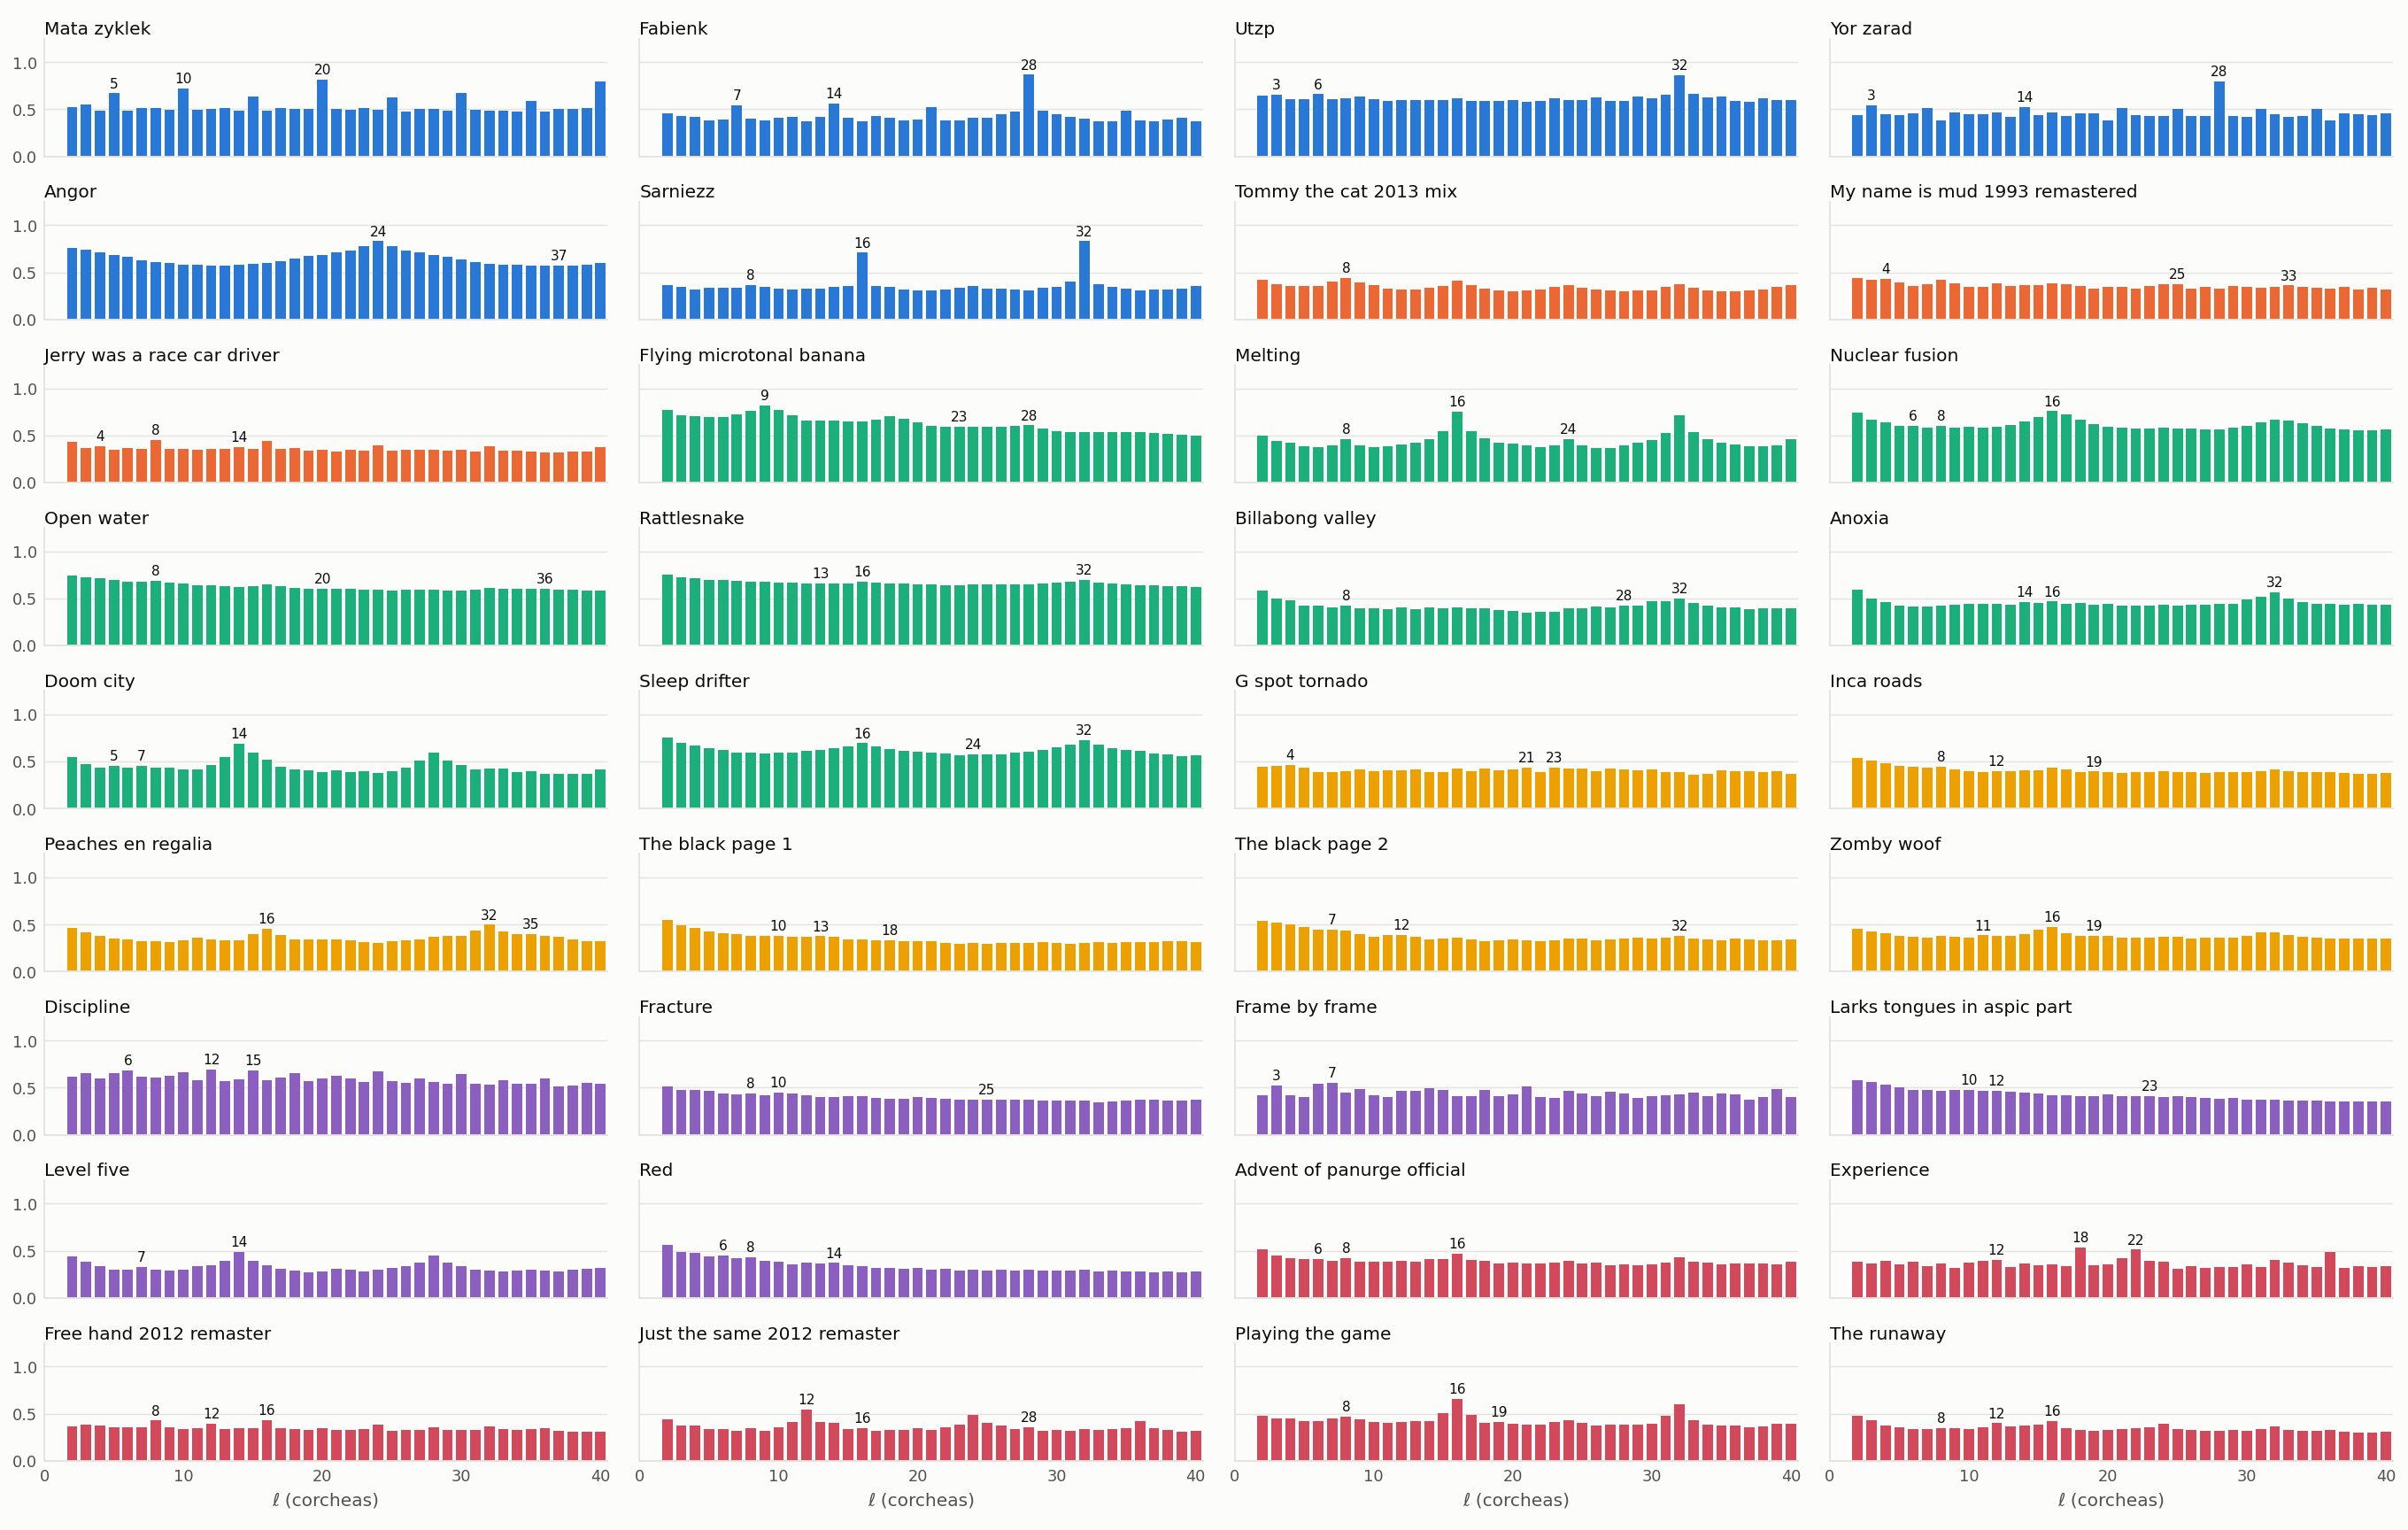
\includegraphics[width=\textwidth]{g_ciclos_metricos.png}
  \caption{Repetición $R(\ell)$ de las 36 canciones (eje $x$: $\ell$ en corcheas; eje $y$: $R$ de 0 a 1). Color por artista: azul, la banda; naranja, Primus; verde, King Gizzard; amarillo, Zappa; violeta, King Crimson; rojo, Gentle Giant. Las cifras sobre las barras son los mejores periodos.}\label{fig:ciclos-todos}
\end{figure}

\begin{figure}[htbp]
  \centering
  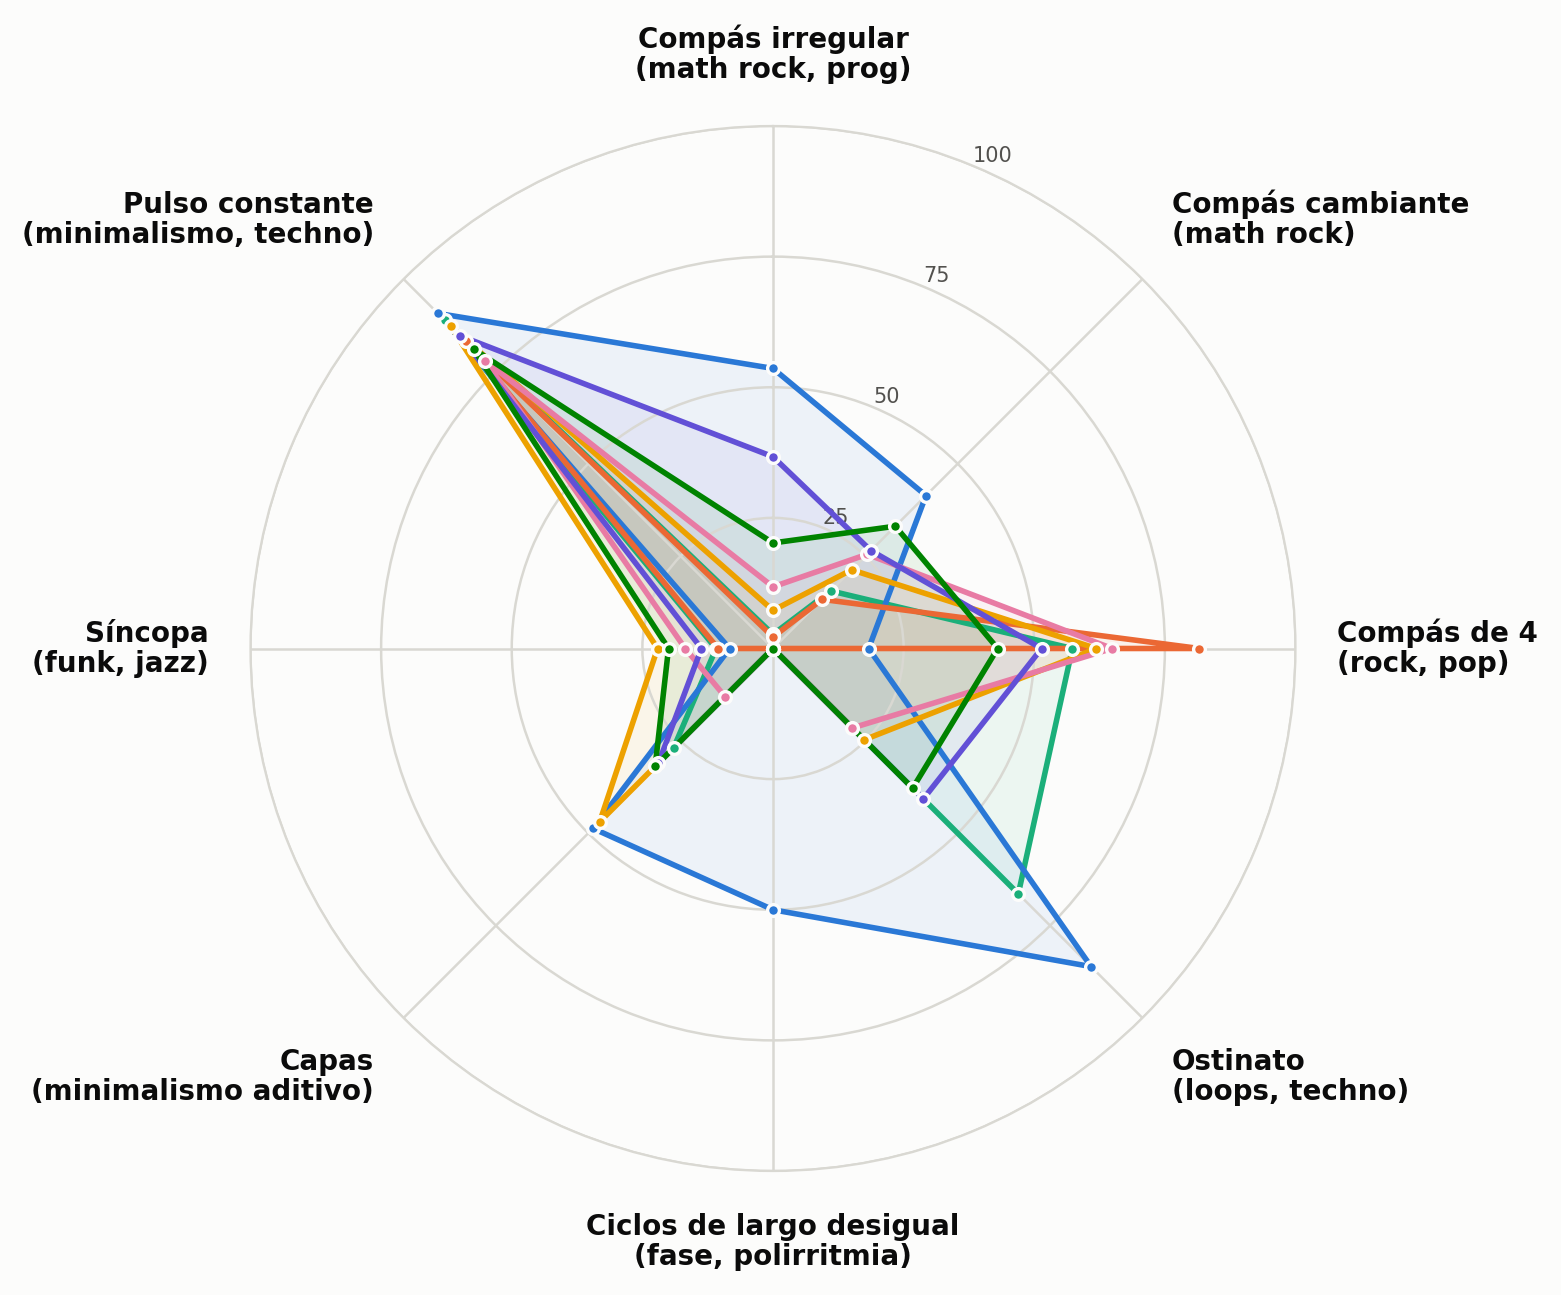
\includegraphics[width=0.55\textwidth]{g_radar_ritmico.png}
  \caption{Perfil rítmico por grupo (mediana, 0--100; más lejos del centro, más presente el rasgo). Verde azulado: la banda (5 canciones); azul: Fabienk, aparte; naranja: Primus; amarillo: King Gizzard; rosa: Zappa; violeta: King Crimson; verde: Gentle Giant.}\label{fig:radar-ritmico}
\end{figure}

\subsection{Bucle contra compás}

El compás que lee la herramienta y el ciclo del riff no siempre coinciden. Para cada compás se busca en qué punto del bucle
cae su primer tiempo (la rotación de la plantilla del bucle que mejor encaja con lo que suena). Si el compás mide lo mismo
que el bucle o lo divide, esa fase queda fija; si mide otra cosa, la fase avanza en escalera, compás a compás; un salto
aislado tras un silencio indica que el riff volvió a entrar por otro punto (figura~\ref{fig:bucle}).

\begin{figure}[htbp]
  \centering
  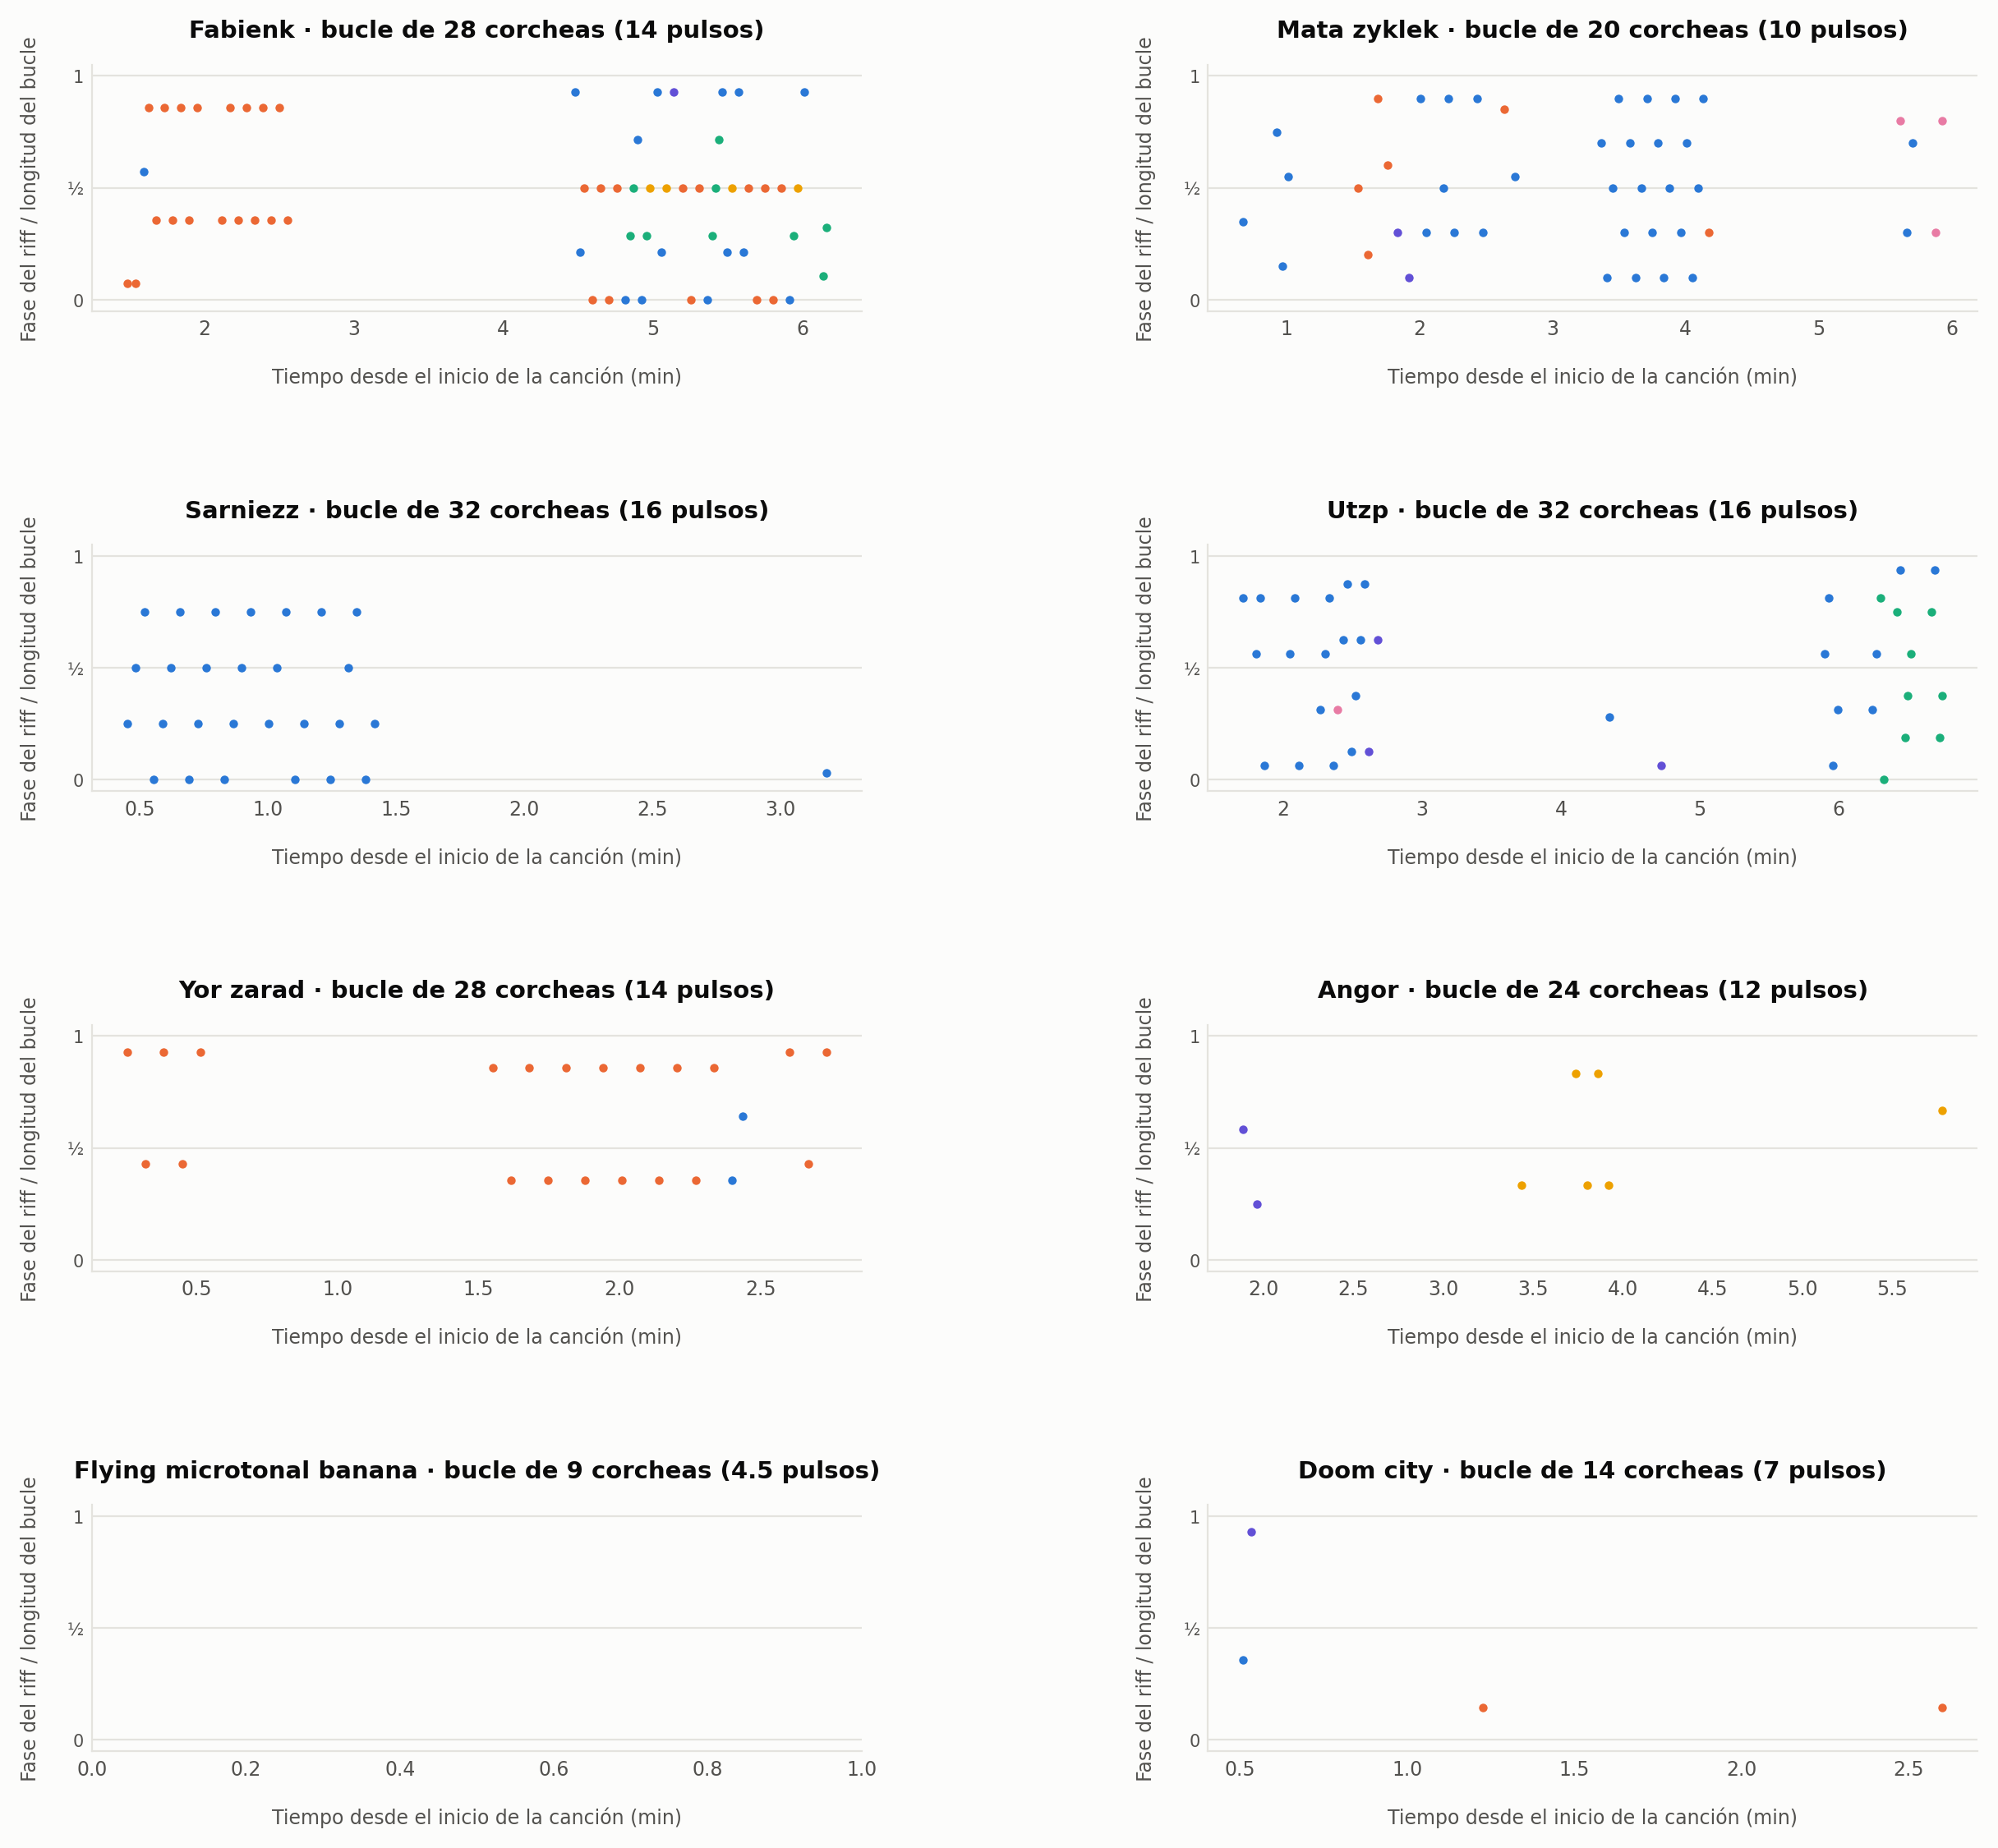
\includegraphics[width=0.92\textwidth]{bucle_compas.png}
  \caption{Fase del riff al inicio de cada compás: cada punto es un compás (eje $x$: minuto; eje $y$: fracción del bucle). Fase fija: compás y bucle coinciden; en escalera: tienen largos distintos; salto aislado: el riff vuelve a entrar tras un silencio. Color: pulsos del compás (verde 3, azul 4, rosa 5, amarillo 6, naranja 7, violeta 8). Las dos últimas son de King Gizzard; en «Flying Microtonal Banana» no queda ningún compás que graficar.}\label{fig:bucle}
\end{figure}

\begin{table}[ht]
  \centering\small
  \caption{Bucle contra compás: fracción de compases que no dividen al bucle ni son múltiplo de él.}\label{tab:bucle}
  \begin{tabular}{@{}lrr@{}}
    \toprule
    Canción & Bucle (corcheas) & Compases que no encajan \\
    \midrule
    Mata Zyklek & 20 & 93\,\% \\
    Fabienk & 28 & 48\,\% \\
    Utzp & 32 & 26\,\% \\
    Angor & 24 & 25\,\% \\
    Yor Zarad & 28 & 9\,\% \\
    Sarniezz & 32 & 0\,\% \\
    \bottomrule
  \end{tabular}
\end{table}

La tabla~\ref{tab:bucle} cuenta, en cada canción, los compases que no encajan. En Mata Zyklek, el 93\,\% no encaja con
el bucle: la herramienta lee la mayor parte de la canción en 4
(compases de 8 corcheas), mientras que el riff dura 20 corcheas. En todos los pasos de un compás al siguiente la fase
avanza exactamente lo que mide el compás, sin saltos: es una escalera regular, como la que produciría un polímetro, un
riff de 5 sobre un pulso de 4, tal como propone Mathémusique \citep{mathemusique2026}. La otra explicación es que la
herramienta lea mal el compás. Los datos no permiten decidir entre las dos, y queda como pregunta para comprobar de oído.
En Sarniezz, en cambio, compás y bucle encajan siempre: todo va en 4.

\section{Síntesis: un híbrido}\label{sec:res-sintesis}

La figura~\ref{fig:clasificacion} reúne los cuatro bloques. Los números de cada casilla muestran de dónde sale el color:
por ejemplo, Sarniezz da 34 en rock solo por el metro, porque su armonía da 0. El 83 de Mata Zyklek en práctica común no
es un parecido real: Kostka-Payne tiene solo 46 piezas y solo armonía, y la armonía de Mata Zyklek es un pedal (89\,\% del
tiempo sobre I y 6\,\% sobre V), un reparto tónica-dominante que tiene cualquier corpus tonal.

\begin{figure}[htbp]
  \centering
  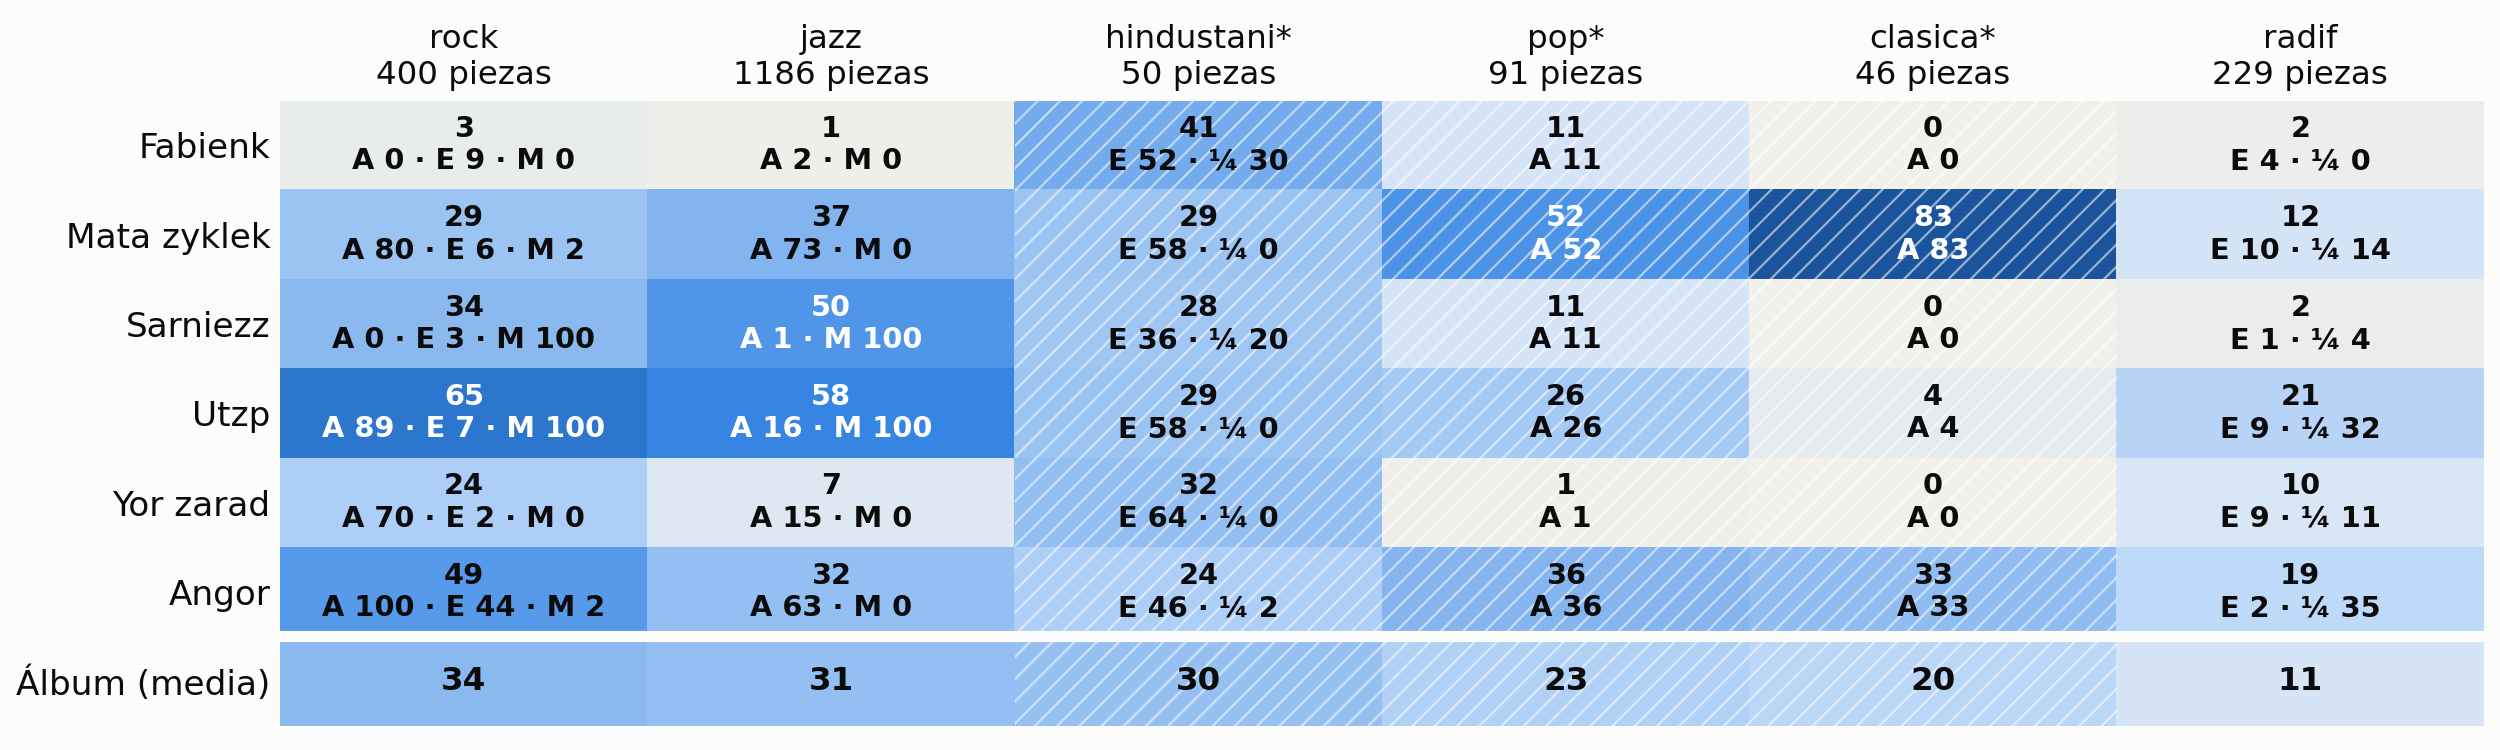
\includegraphics[width=\textwidth]{g_clasificacion_detalle.png}
  \caption{Clasificación del álbum por corpus. Color: percentil medio de tipicidad, de blanco (atípica) a azul oscuro (muy típica). En cada casilla, la media y el percentil de cada bloque (A armonía, E escala, \cuarto{} cuartos de tono, M metro). Asterisco y rayado: corpus de menos de 100 piezas, fuera del veredicto. En los encabezados, «clasica» es la práctica común y «hindustani», el corpus indostánico.}\label{fig:clasificacion}
\end{figure}

Las mismas medidas para las 36 canciones, bloque por bloque, están en el apéndice (figuras~\ref{fig:g-bloques}
y~\ref{fig:g-bloques-sintesis}).

Si se cuenta qué corpus se parece más en cada bloque (figura~\ref{fig:ganadores}), el rock gana 8 de 24, la mitad de
ellos en armonía (4 de 6 canciones): es rock modal. El radif gana 7, sobre todo en cuartos de tono. En los 9 restantes ningún corpus llega al
percentil 5. La tabla~\ref{tab:veredictos} da el veredicto de cada canción.

\begin{figure}[htbp]
  \centering
  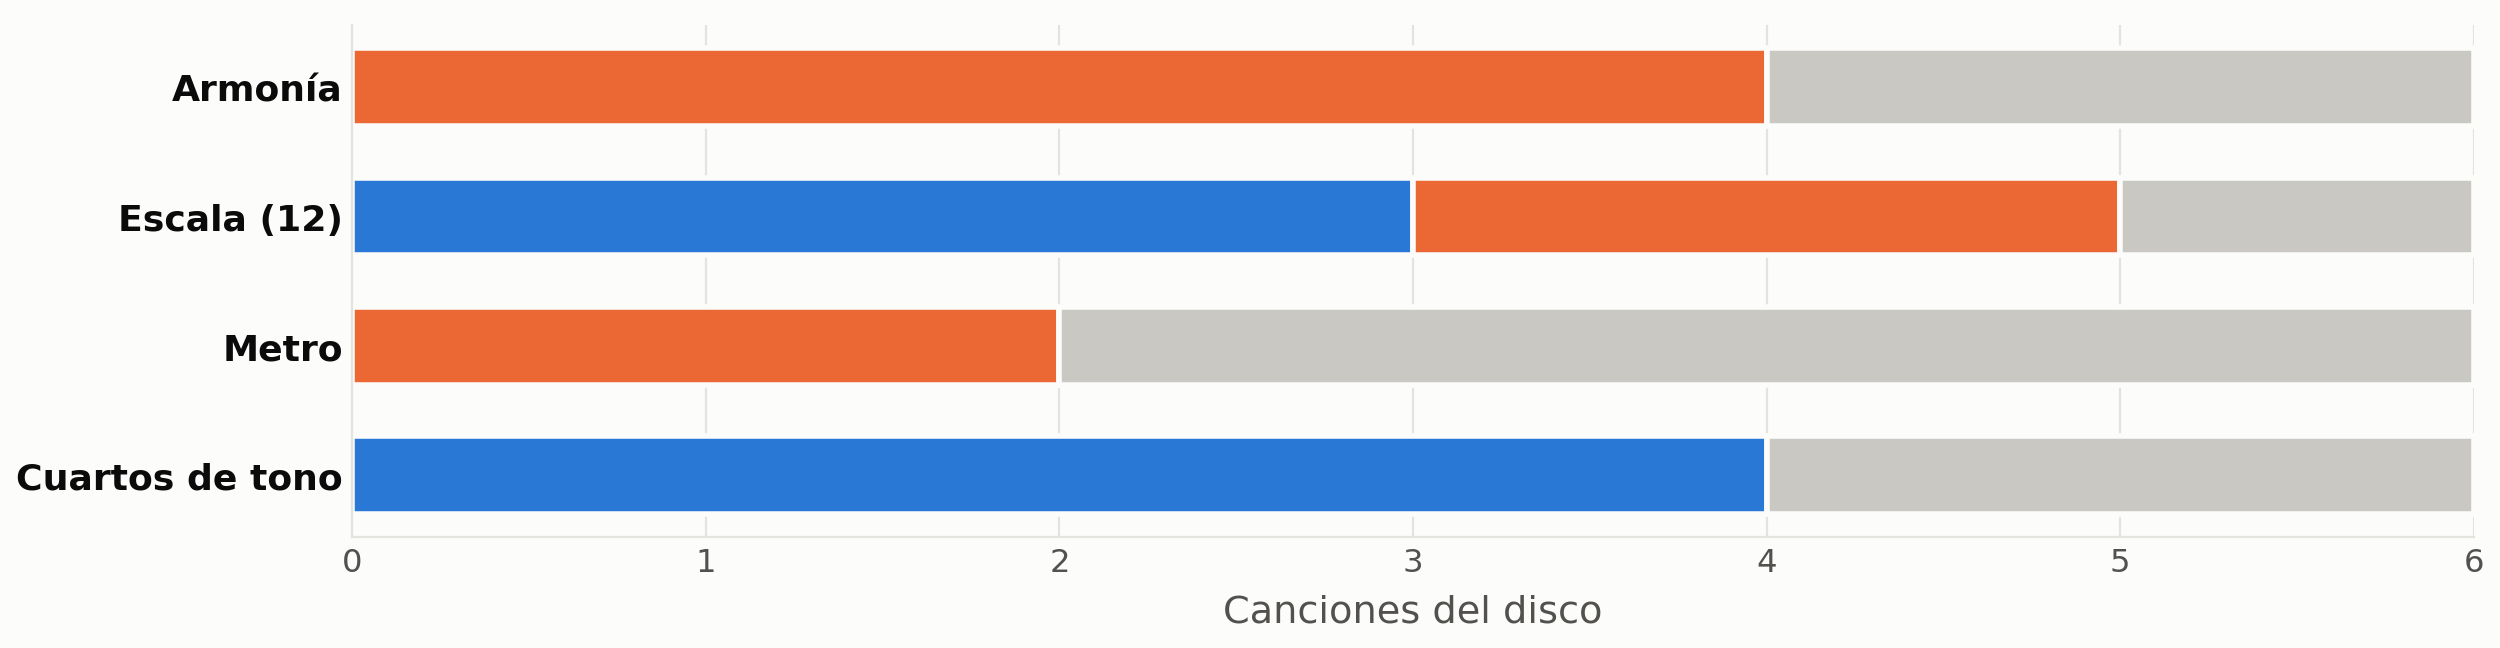
\includegraphics[width=0.85\textwidth]{3c_sintesis_corpus_por_bloque.png}
  \caption{Qué corpus gana cada bloque, en número de canciones. Azul: radif (7); naranja: rock (8); gris: sin vecino, ningún corpus llega al percentil 5 (9).}
  \label{fig:ganadores}
\end{figure}

\begin{table}[ht]
  \centering\small
  \caption{Veredicto del test por bloques (corpus con 100 piezas o más).}\label{tab:veredictos}
  \begin{tabularx}{\textwidth}{@{}l>{\raggedright\arraybackslash}X@{}}
    \toprule
    Canción & Veredicto \\
    \midrule
    Mata Zyklek & Rasgo sin vecino: metro \\
    Fabienk & Rasgo sin vecino: armonía, cuartos de tono y metro \\
    Sarniezz & Rasgo sin vecino: armonía, escala y cuartos de tono \\
    Yor Zarad & Rasgo sin vecino: metro \\
    Angor & Rasgo sin vecino: metro \\
    Utzp & Síntesis de lenguajes existentes \\
    \bottomrule
  \end{tabularx}
\end{table}

En ningún caso el veredicto es «estilo existente»: ningún corpus tiene los cuatro bloques, y ninguno explica la
combinación. El vecino más cercano en conjunto es King Gizzard: en armonía, Angor es idéntica a «Flying Microtonal
Banana», porque ambas son un pedal sobre I. Sarniezz y Fabienk no tienen vecino ni siquiera ahí.

\section{Análisis por canción}\label{sec:por-cancion}

Esta sección reúne, canción por canción, lo que la herramienta mide en el álbum. Para cada una se muestran una página del
tabroll con la armonía en 24-EDO y el mapa de ciclos del looper. En el tabroll, las filas son las 24 clases por octava
(las filas «¼» son los cuartos de tono), cada recuadro es un compás con su número de pulsos arriba y su acorde abajo
(cifrado romano, función y nombre; entre paréntesis, los compases de baja confianza), y los anillos dorados marcan la
columna principal del compás. En el mapa de ciclos, cada barra es un tramo en que una voz repite un ciclo, con su letra y
su periodo, y la curva inferior estima cuántas capas del looper suenan.

La tabla~\ref{tab:resumen-canciones} resume las medidas principales.

\begin{table}[ht]
  \centering\footnotesize\setlength{\tabcolsep}{4pt}
  \caption{Resumen por canción. «Conf.»: porcentaje del tiempo en compases confiables. «Ciclo»: mejor periodo de
  $R(\ell)$ en corcheas.}\label{tab:resumen-canciones}
  \begin{tabular}{@{}lrrlllrr@{}}
    \toprule
    Canción & BPM & Conf. & Centro & Modo (2, 3, 6, 7) & \shortstack{Fundamental\\más usada} & \shortstack{\cuarto{} de\\tono} & Ciclo \\
    \midrule
    Mata Zyklek & 94 & 78\,\% & Sol & \fl2+, 3, \fl6+, \fl7 & I (89\,\%) & 23.9\,\% & 20 \\
    Fabienk & 129 & 85\,\% & Mi & 2, \fl3, 6, \fl7 & I, \fl VII, \fl III & 14.2\,\% & 28 \\
    Sarniezz & 115 & 58\,\% & Mi & 2, \fl3, 6, \fl7 & \fl III (40\,\%) & 25.3\,\% & 32 \\
    Yor Zarad & 108 & 75\,\% & Sol & \fl2+, 3, \fl6+, \fl7 & I (85\,\%) & 16.8\,\% & 28 \\
    Utzp & 129 & 82\,\% & Mi & \fl2+, \fl3, \fl6+, \fl7 & I (96\,\%) & 11.1\,\% & 32 \\
    Angor & 99 & 88\,\% & Sol & \fl2+, \fl3, 6, \fl7 & I (100\,\%) & 5.0\,\% & 24 \\
    \bottomrule
  \end{tabular}
\end{table}

Los modos confirman las dos familias de la sección~\ref{sec:res-melodia}. Mata Zyklek y Yor Zarad tienen la misma
descripción: \fl2+, 3, \fl6+, \fl7. Es un frigio dominante (\fl2, 3, \fl6, \fl7) con la segunda y la sexta subidas un
cuarto de tono, es decir, con una segunda neutra en lugar de la aumentada; en doce notas se leería como hijaz, y eso
explica la comparación de David Bennett. Utzp es el mismo esquema sobre un frigio menor (\fl3). Fabienk y Sarniezz son
dóricos (2, \fl3, 6, \fl7), con los cuartos de tono en la melodía (7+, 6+, \fl3+) y no en el modo de los acordes.

\FloatBarrier
\subsection{Mata Zyklek}

La figura~\ref{fig:mata} muestra una página del tabroll24 y el mapa de ciclos; la tarjeta y la tira de ciclos son las figuras~\ref{fig:tarjeta-mata} y~\ref{fig:tira-mata}, y su círculo armónico está en el apéndice (figura~\ref{fig:circulos1}).

\begin{figure}[p]
  \centering
  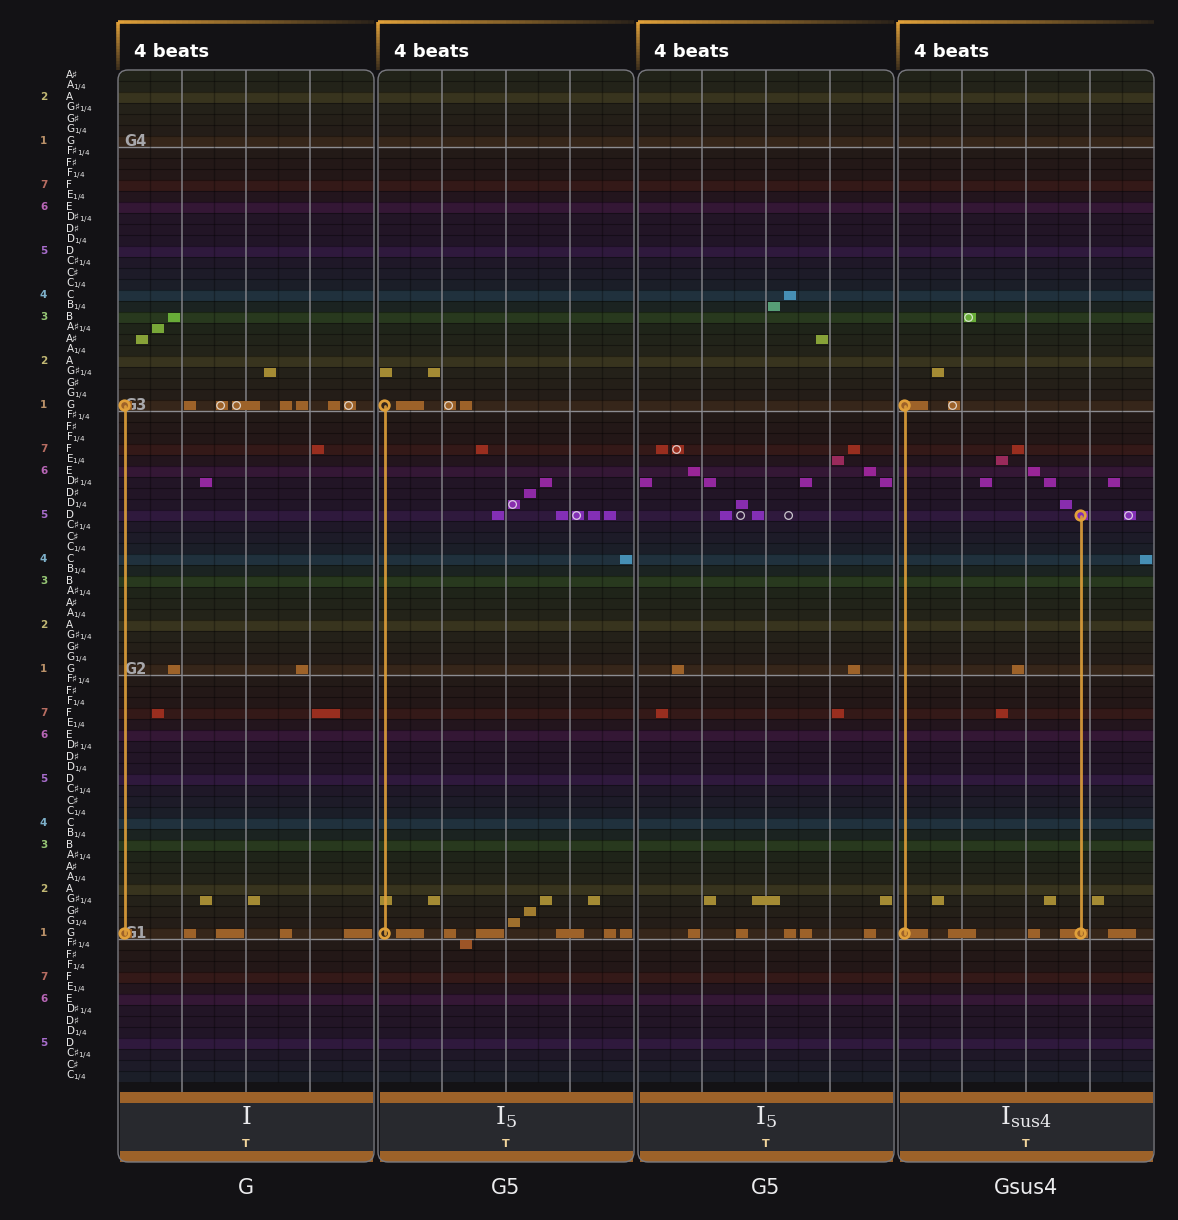
\includegraphics[width=0.78\textwidth]{mata_zyklek_tabroll24.png}\\[0.5em]
  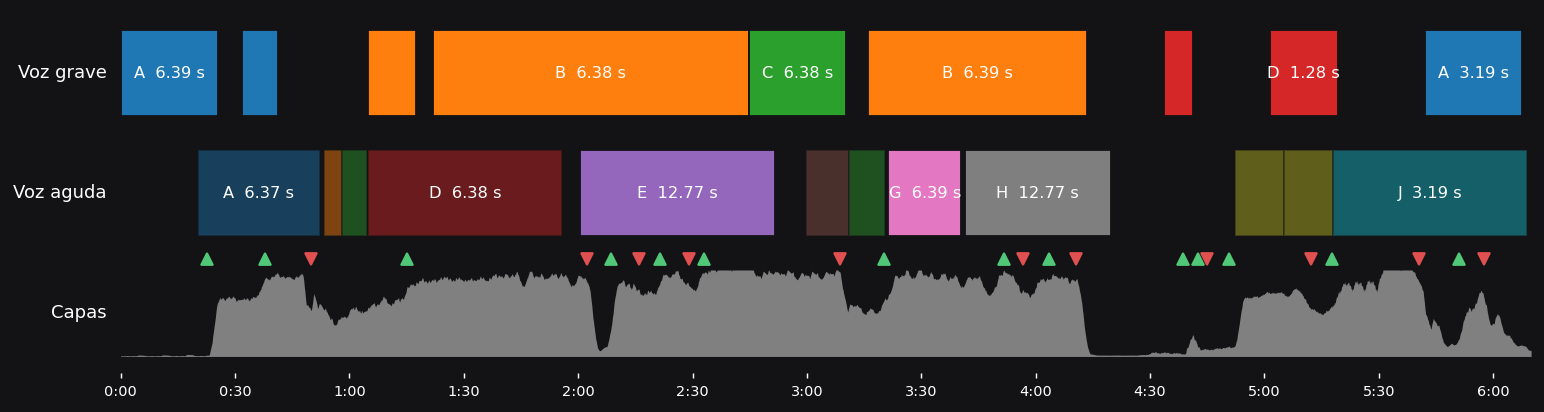
\includegraphics[width=\textwidth]{mata_zyklek_mapa_ciclos.png}
  \caption{Mata Zyklek. Arriba, una página del tabroll24: notas en 24-EDO (filas «¼», cuartos de tono), pulsos de cada compás («beats») y acorde debajo. Abajo, mapa de ciclos: cada barra es un tramo repetido de una voz, con su letra y su periodo; la curva gris estima las capas del looper (triángulos verdes: entra una capa; rojos: sale).}\label{fig:mata}
\end{figure}

\paragraph{Armonía.} Es un pedal: la fundamental está en I el 89\,\% del tiempo (quinta sola el 53\,\% y tríada mayor el
34\,\%), con V (6\,\%), \fl2+ (3\,\%) y \fl VII (2\,\%). Entre compases confiables solo hay dos cambios, I5 $\to$ Vsus4
$\to$ I: una cadencia auténtica. Con todos los compases aparece además, en la introducción, el vaivén \fl II+5
$\leftrightarrow$ \fl VII, que la partitura confirma pero que tiene confianza baja (0.14 a 0.44). La introducción está
centrada en Sol\sh+ (\fl2+): la canción empieza sobre el cuarto de tono y llega a Sol.

\paragraph{Melodía.} Es la canción con más tiempo en cuartos de tono como grado (19.1\,\%). Los dos grados principales son
\fl2+ (11.3\,\% del tiempo de la melodía) y \fl6+ (5.2\,\%); \fl2+ y 1+ aparecen en todas las vueltas del ciclo. En el bajo,
lo que más varía entre vueltas es Sol\sh+ $\leftrightarrow$ Sol: la fundamental y su segunda neutra (\fl2+), tres cuartos de tono más arriba.

\paragraph{Metro y comparación.} El riff se repite cada 20 corcheas (dos compases de 5/4, $R = 0.82$). En el test por bloques
su armonía tiene vecinos en el rock (percentil 79.5): el rock tiene piezas de pedal, aunque frente al \emph{centro} del rock
quede lejos (12 en la matriz). Lo que no tiene vecino es el metro.

\FloatBarrier
\subsection{Fabienk}

La figura~\ref{fig:fabienk-tarjeta} reúne la tarjeta y la tira de ciclos; la figura~\ref{fig:fabienk}, una página del tabroll24 y el mapa de ciclos.

\begin{figure}[!h]
  \centering
  \begin{subfigure}[c]{0.42\textwidth}\centering
    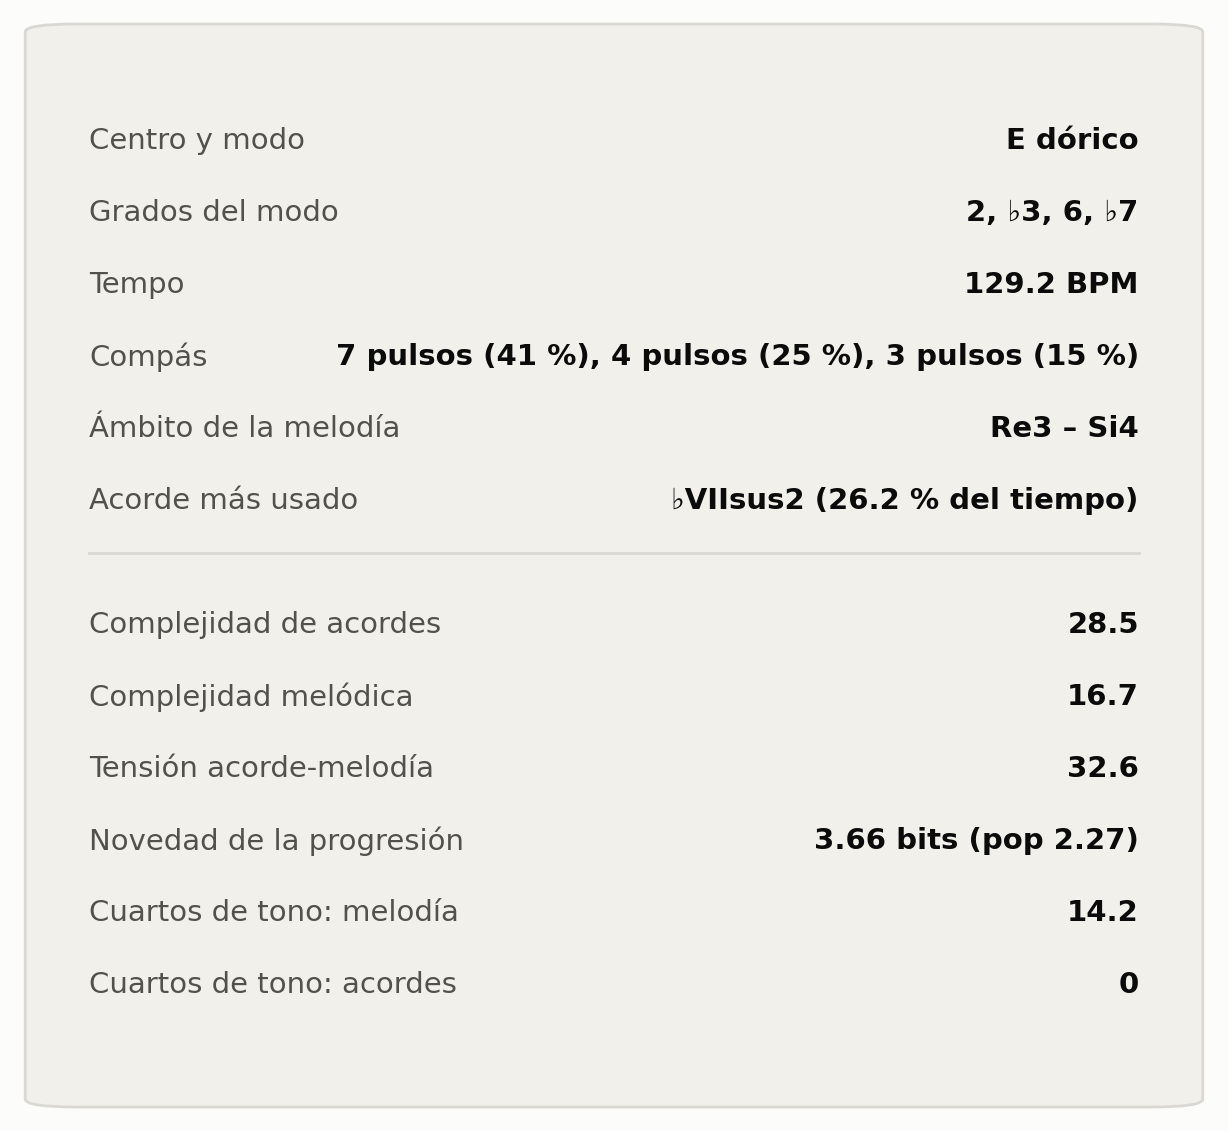
\includegraphics[width=\linewidth]{fabienk_tarjeta.png}\caption{Tarjeta.}
  \end{subfigure}\hfill
  \begin{subfigure}[c]{0.55\textwidth}\centering
    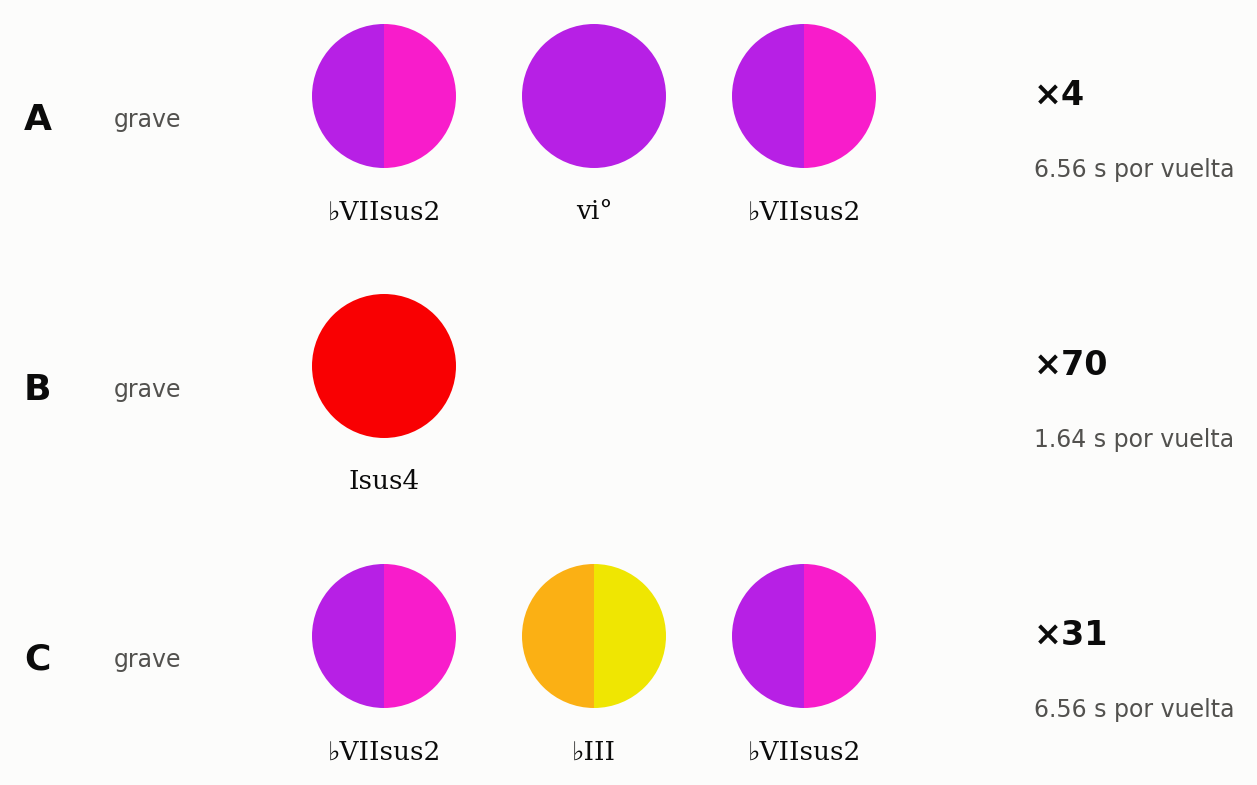
\includegraphics[width=\linewidth]{fabienk_tira_de_ciclos.png}\caption{Ciclos repetidos.}
  \end{subfigure}
  \caption{Fabienk: tarjeta de medidas crudas (izquierda) y tira de ciclos (derecha; cada fila es un ciclo de la voz indicada, grave o aguda; color = grado de la fundamental, $\times$ = vueltas, s = duración de cada vuelta). Centro Mi, modo 2, \fl3, 6, \fl7; compases confiables: 84.7\,\%; acierto F 45.4 en la melodía y 81.6 en la fundamental.}\label{fig:fabienk-tarjeta}
\end{figure}

\begin{figure}[p]
  \centering
  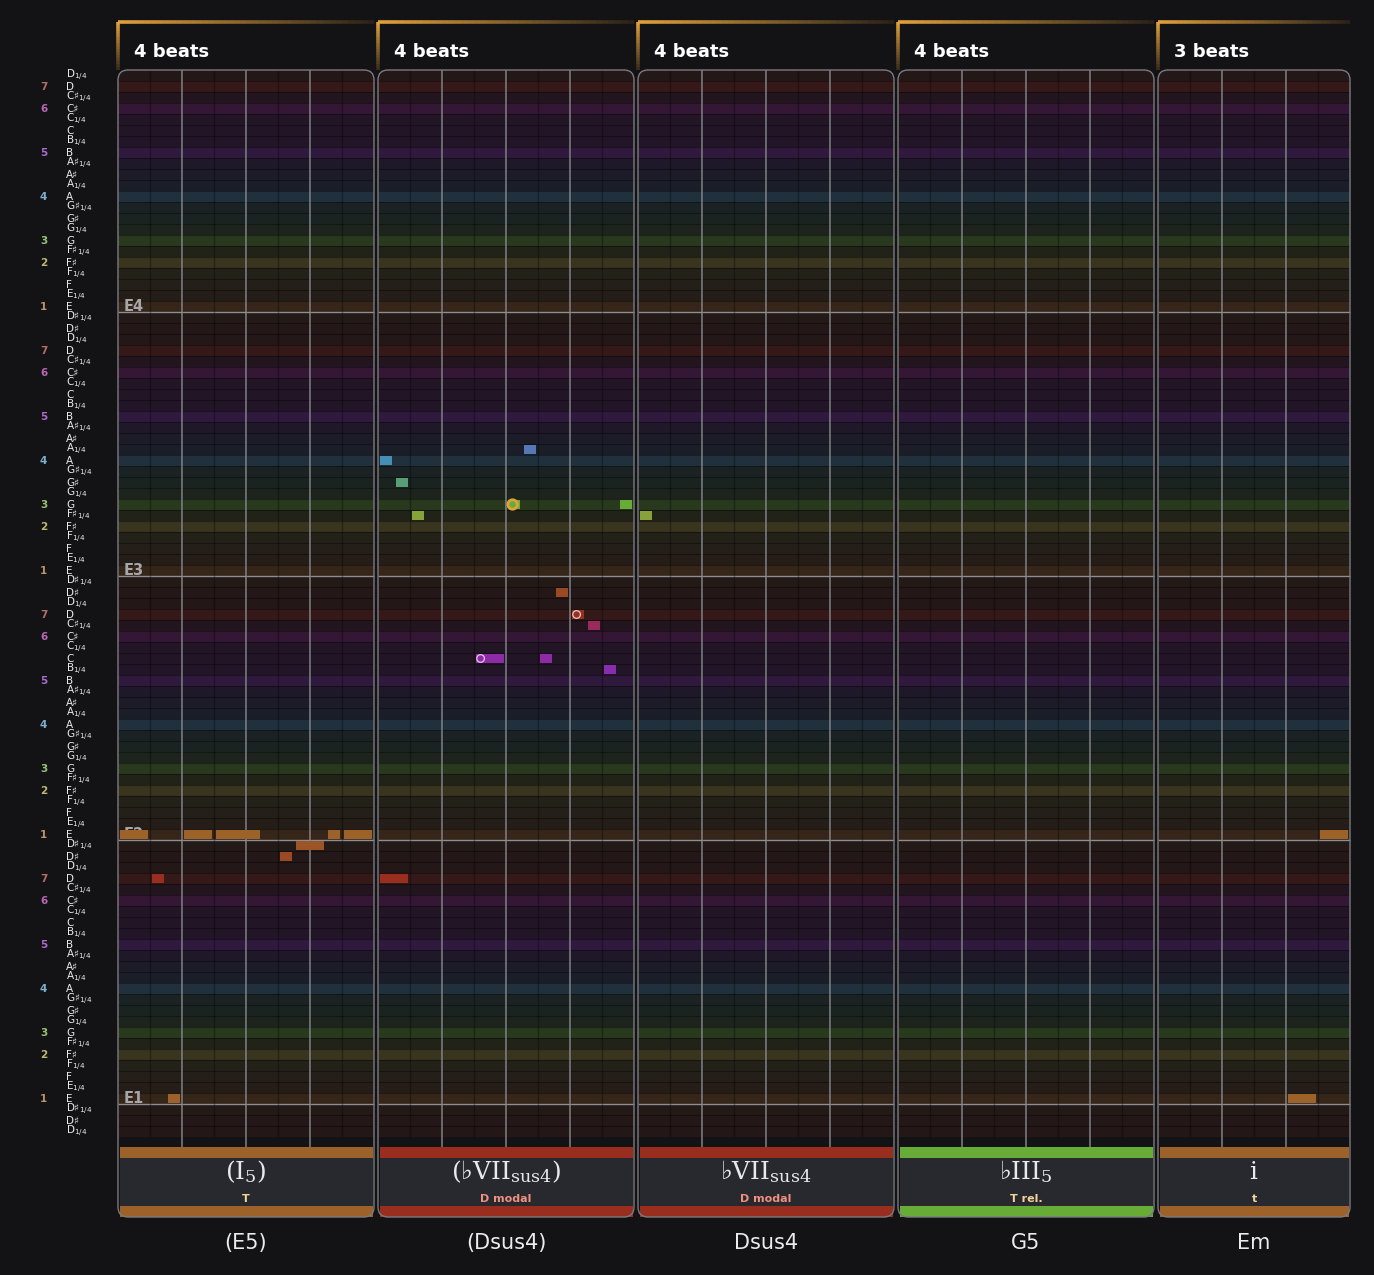
\includegraphics[width=0.7\textwidth]{fabienk_tabroll24.png}\\[0.5em]
  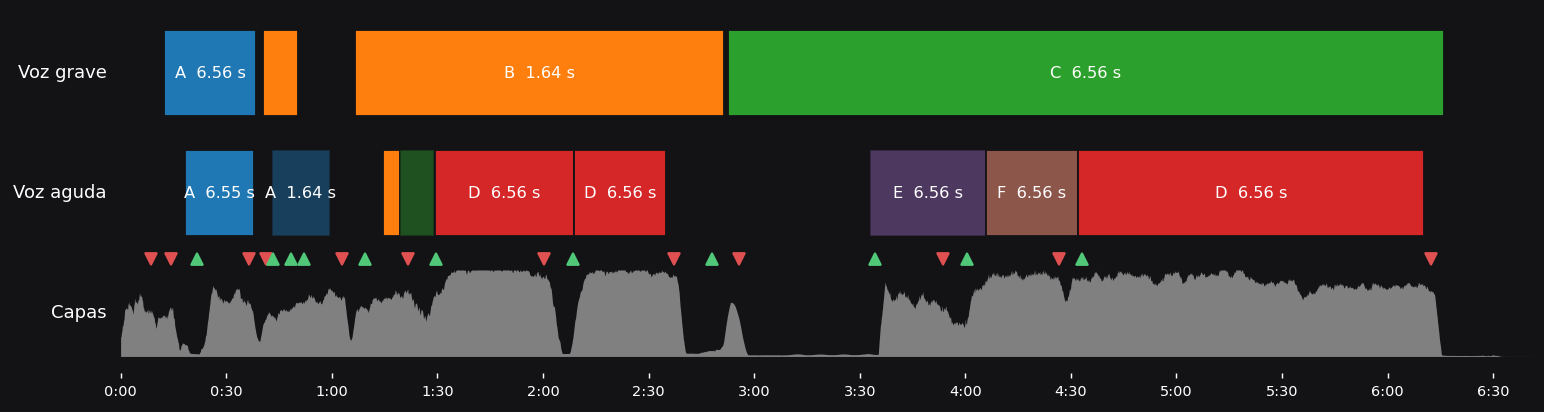
\includegraphics[width=\textwidth]{fabienk_mapa_ciclos.png}
  \caption{Fabienk: una página del tabroll24 (arriba) y el mapa de ciclos (abajo); misma lectura que la figura~\ref{fig:mata}.}\label{fig:fabienk}
\end{figure}

\paragraph{Armonía.} Es la canción con más movimiento armónico: 86 cambios entre compases confiables, la mitad por quintas
(51\,\%), seguidos de segundas (28\,\%) y terceras abajo (21\,\%). Tres fundamentales se reparten el tiempo casi por igual:
I (34\,\%), \fl VII (33\,\%) y \fl III (29\,\%). Las progresiones más frecuentes son \fl VII $\to$ \fl III y el vaivén
\fl III $\leftrightarrow$ \fl VIIsus2; aparece la cadencia modal \fl VII--I. El acorde más usado es \fl VIIsus2 (26\,\%).
El centro es dudoso (margen 0.015): el bajo descansa en \fl VII, y por eso se usa el centro que coincide con el oído, Mi.

\paragraph{Melodía.} Los cuartos de tono ocupan el 14.2\,\% de la melodía, concentrados en 7+ (4.6\,\%) y 6+ (4.3\,\%); 6+
aparece en todas las vueltas del ciclo.

\paragraph{Metro.} El ciclo dura 28 corcheas, dos compases de 7/4 ($R = 0.87$, empatado con Utzp como el más estable del álbum). La canción pasa
el 53\,\% del tiempo en compases de 7, el 18\,\% en 4 y el 9\,\% en 3. La tarjeta de la figura~\ref{fig:fabienk-tarjeta}
cuenta compases y no tiempo: 41\,\% de 7, 25\,\% de 4 y 15\,\% de 3; como el compás de 7 es el más largo, pesa más en
tiempo que en número. Sin vecino en armonía, cuartos de tono y metro.

\clearpage
\subsection{Sarniezz}

La figura~\ref{fig:sarniezz-tarjeta} reúne la tarjeta y la tira de ciclos; la figura~\ref{fig:sarniezz}, una página del tabroll24 y el mapa de ciclos.

\begin{figure}[!h]
  \centering
  \begin{subfigure}[c]{0.42\textwidth}\centering
    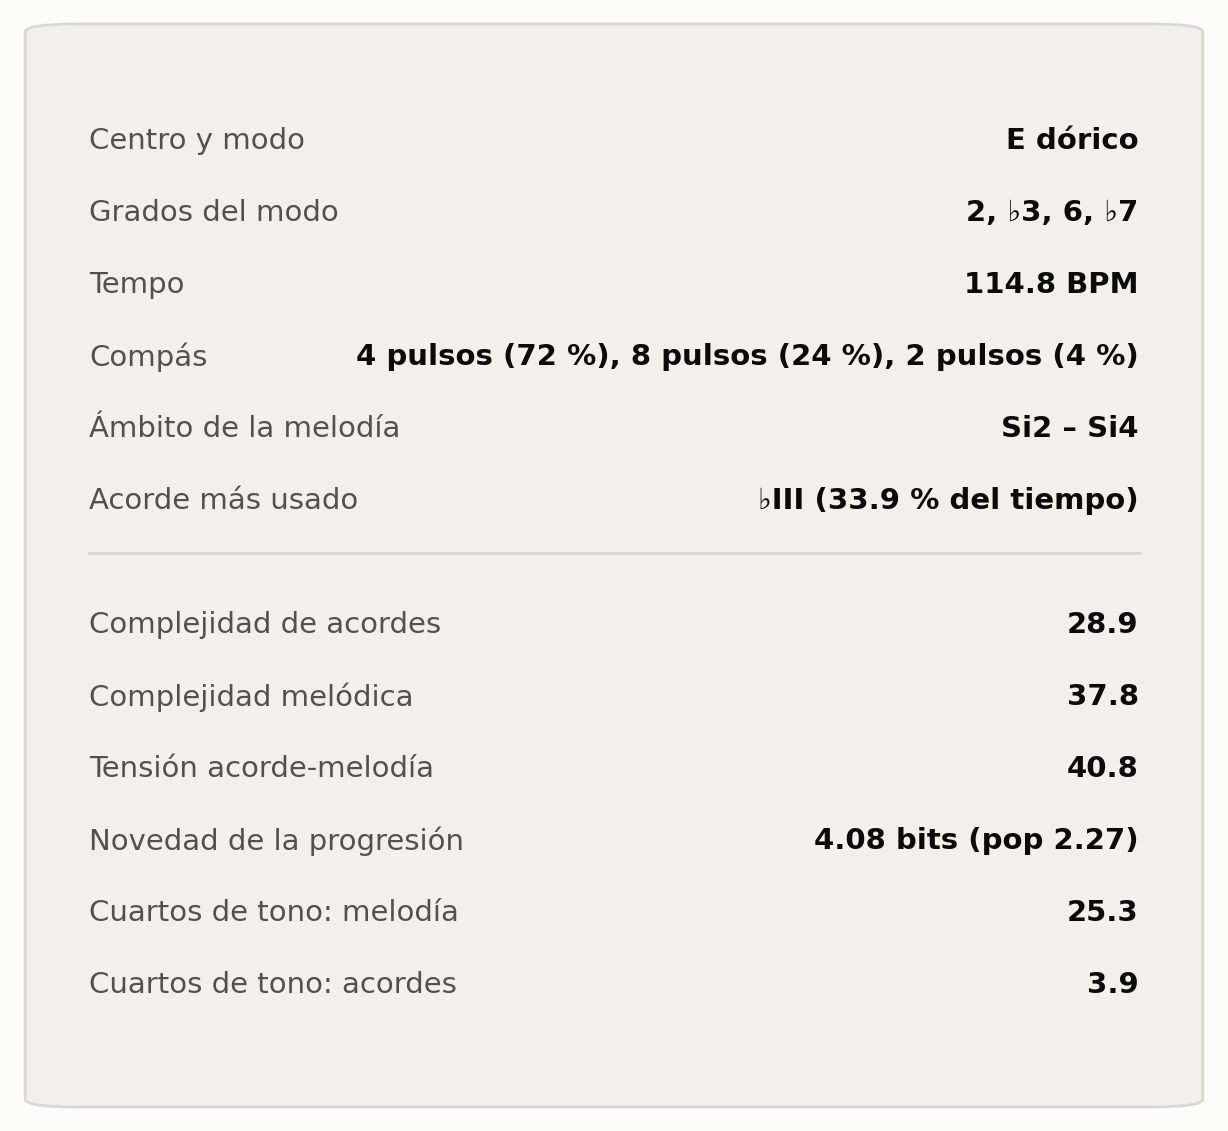
\includegraphics[width=\linewidth]{sarniezz_tarjeta.png}\caption{Tarjeta.}
  \end{subfigure}\hfill
  \begin{subfigure}[c]{0.55\textwidth}\centering
    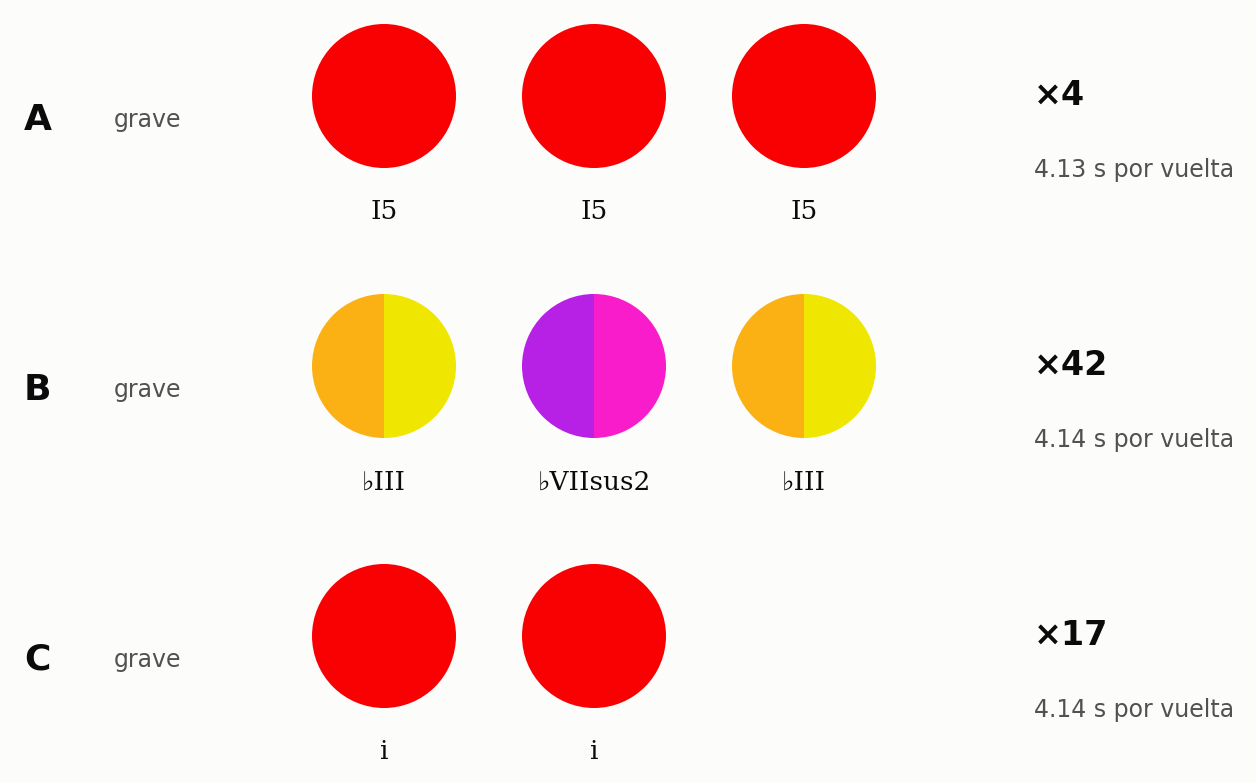
\includegraphics[width=\linewidth]{sarniezz_tira_de_ciclos.png}\caption{Ciclos repetidos.}
  \end{subfigure}
  \caption{Sarniezz: tarjeta y tira de ciclos; misma lectura que la figura~\ref{fig:fabienk-tarjeta}. Centro Mi, modo 2, \fl3, 6, \fl7; compases confiables: 57.6\,\%; acierto F 44.9 en la melodía y 57.5 en la fundamental.}\label{fig:sarniezz-tarjeta}
\end{figure}

\begin{figure}[p]
  \centering
  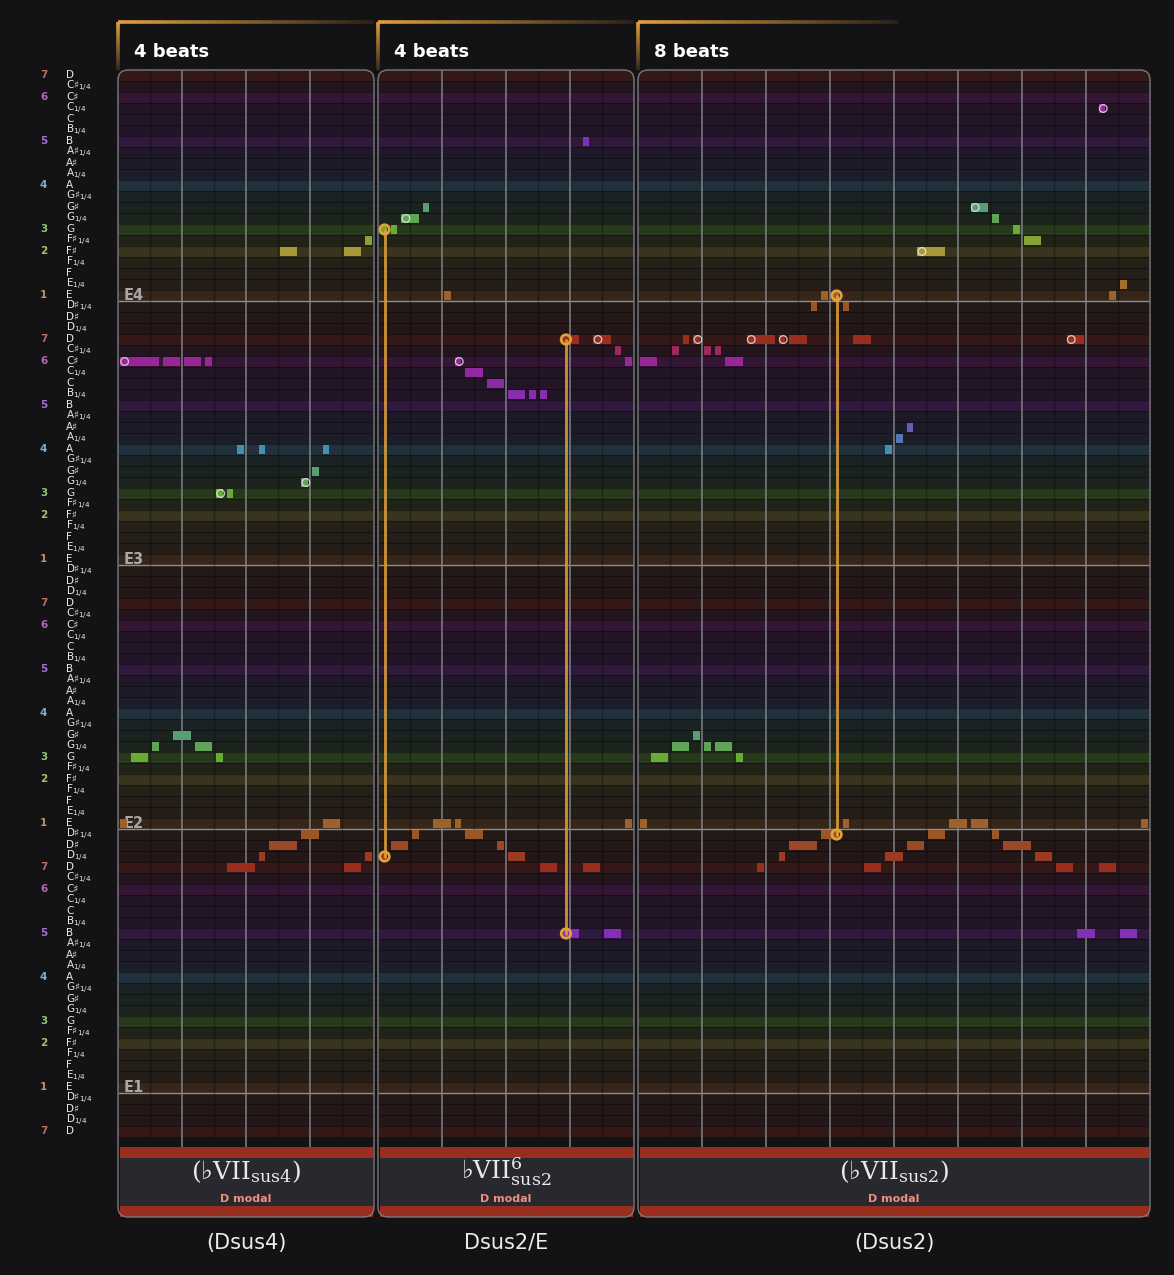
\includegraphics[width=0.7\textwidth]{sarniezz_tabroll24.png}\\[0.5em]
  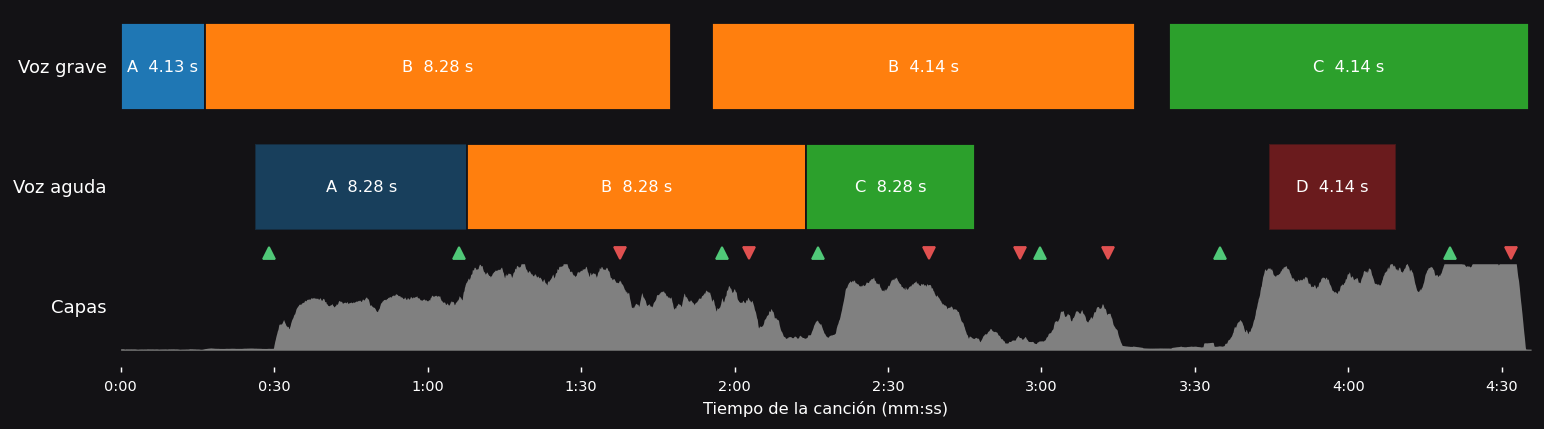
\includegraphics[width=\textwidth]{sarniezz_mapa_ciclos.png}
  \caption{Sarniezz: una página del tabroll24 (arriba) y el mapa de ciclos (abajo); misma lectura que la figura~\ref{fig:mata}.}\label{fig:sarniezz}
\end{figure}

\paragraph{Armonía.} La fundamental más usada no es la tónica sino \fl III (40\,\%), seguida de \fl VII (29\,\%) y I
(24\,\%). El vaivén \fl III $\leftrightarrow$ \fl VIIsus2 se repite 31 veces. El 59\,\% de los cambios va por quintas, pero
el 9\,\% es microtonal. Según los ejes de Lendvai, el 24\,\% de los cambios de la partitura queda dentro del eje de tónica
(I $\leftrightarrow$ \fl III), una sustitución y no un movimiento por quintas. Los centros por tramo muestran por qué el
centro es difícil: los tramos B giran sobre Re (\fl7) y el C sobre Sol (\fl3), y Mi solo ocupa el 6\,\% de los tramos. Es
la canción con menos compases confiables (58\,\%) y con la armonía menos acertada (57.5\,\%).

\paragraph{Melodía.} Tiene la mayor proporción de cuartos de tono (25.3\,\%) pero la menor concentración (48\,\%):
7+ (6.4\,\%), \fl3+ (5.9\,\%), \fl7+ (3.5\,\%) y 5+ (2.9\,\%). \fl3+ aparece en todas las vueltas y 7+ y 5+ en el 88\,\%.
Es un riff cromático de cuartos de tono, no una escala con dos grados neutros.

\paragraph{Metro.} Va en 4: el ciclo dura 32 corcheas. Sin vecino en armonía, escala y cuartos de tono.

\clearpage
\subsection{Yor Zarad}

La figura~\ref{fig:yor_zarad-tarjeta} reúne la tarjeta y la tira de ciclos; la figura~\ref{fig:yor}, una página del tabroll24 y el mapa de ciclos.

\begin{figure}[!h]
  \centering
  \begin{subfigure}[c]{0.42\textwidth}\centering
    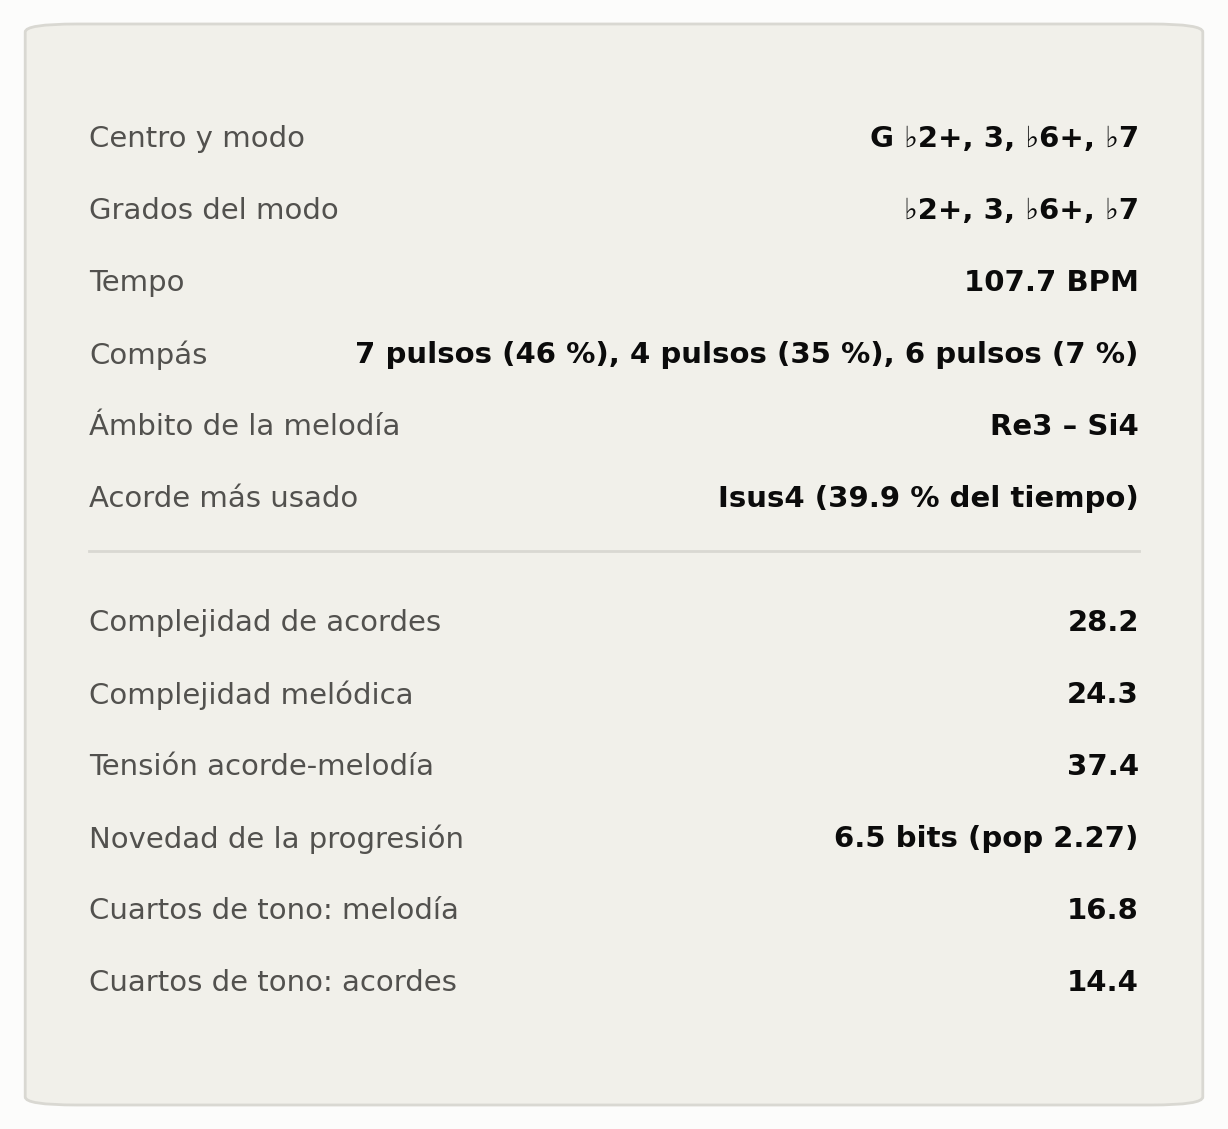
\includegraphics[width=\linewidth]{yor_zarad_tarjeta.png}\caption{Tarjeta.}
  \end{subfigure}\hfill
  \begin{subfigure}[c]{0.55\textwidth}\centering
    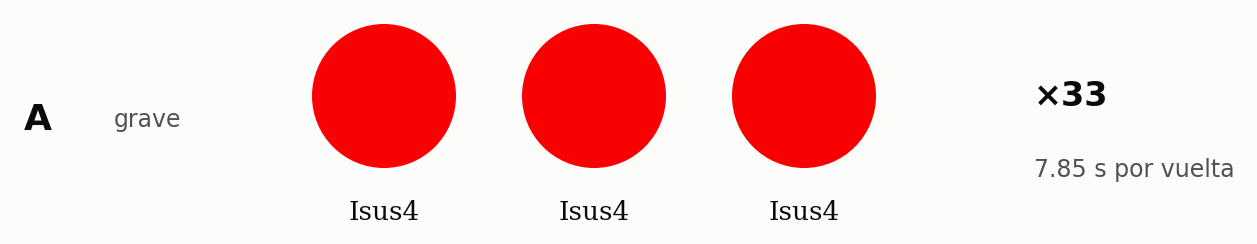
\includegraphics[width=\linewidth]{yor_zarad_tira_de_ciclos.png}\caption{Ciclos repetidos.}
  \end{subfigure}
  \caption{Yor Zarad: tarjeta y tira de ciclos; misma lectura que la figura~\ref{fig:fabienk-tarjeta}. Centro Sol, modo \fl2+, 3, \fl6+, \fl7; compases confiables: 75.2\,\%; acierto F 36.8 en la melodía.}\label{fig:yor_zarad-tarjeta}
\end{figure}

\begin{figure}[p]
  \centering
  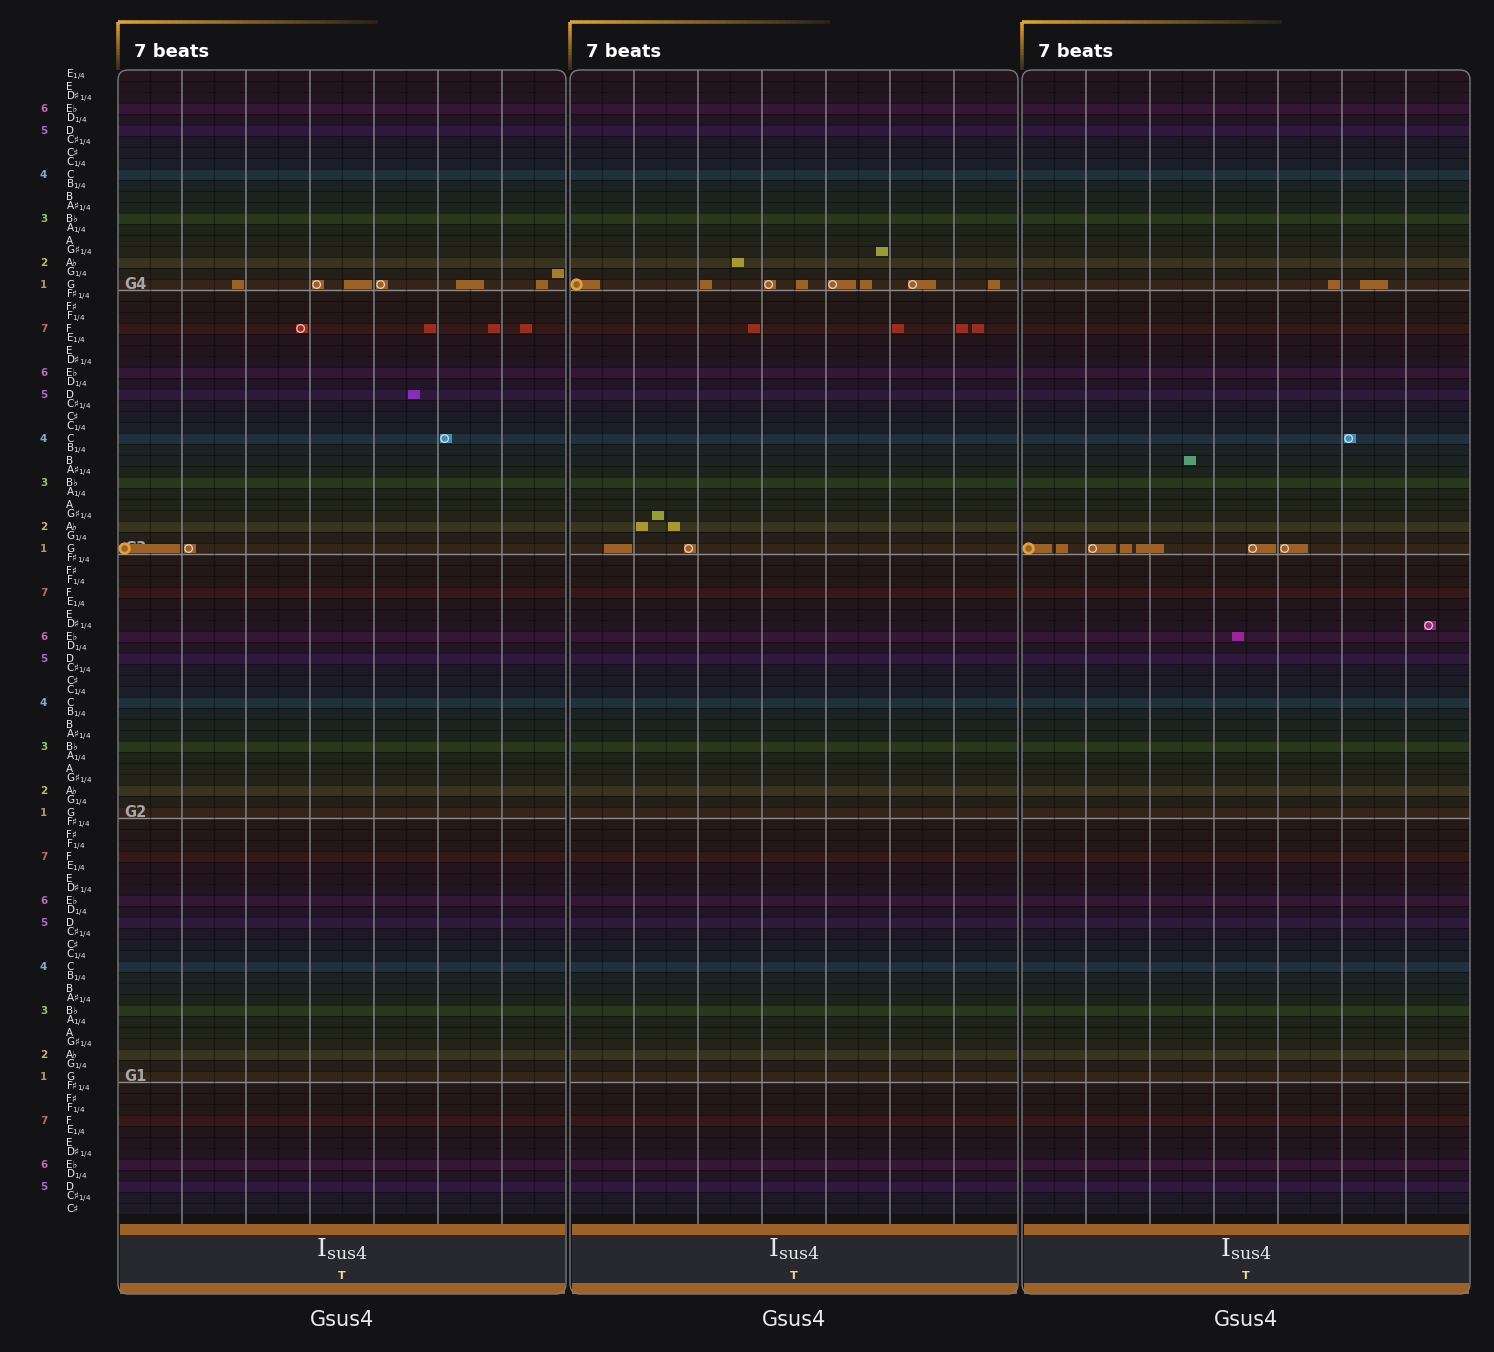
\includegraphics[width=0.75\textwidth]{yor_zarad_tabroll24.png}\\[0.5em]
  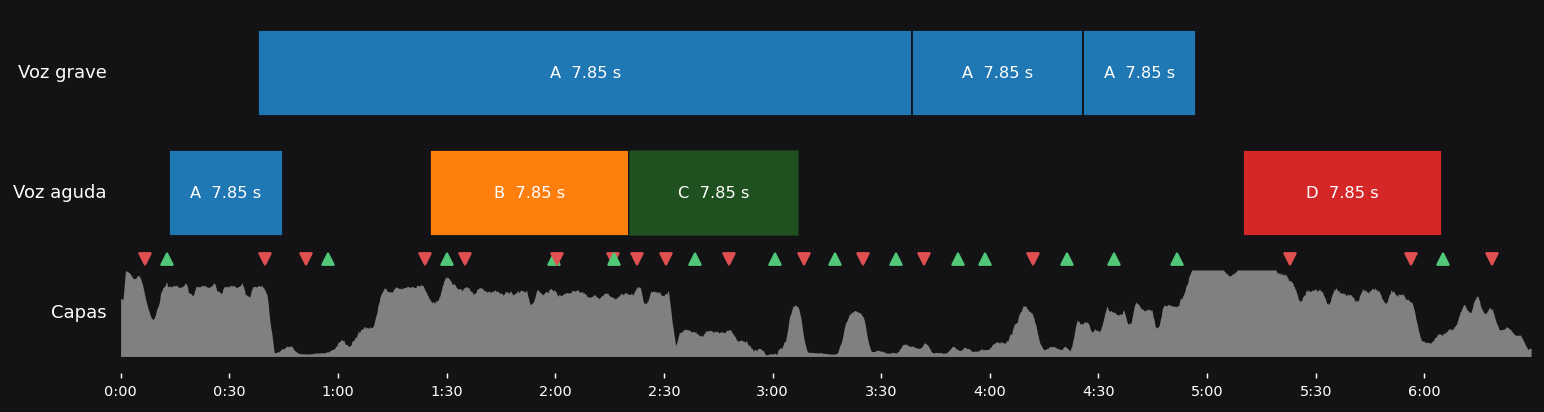
\includegraphics[width=\textwidth]{yor_zarad_mapa_ciclos.png}
  \caption{Yor Zarad: una página del tabroll24 (arriba) y el mapa de ciclos (abajo); misma lectura que la figura~\ref{fig:mata}.}\label{fig:yor}
\end{figure}

\paragraph{Armonía.} La fundamental está en I el 85\,\% del tiempo y en \fl2+ el 13\,\%: los 11 cambios entre compases
confiables son microtonales, todos entre I y \fl II+5 (el vaivén I5 $\leftrightarrow$ \fl II+5 aparece 6 veces). Es decir,
la armonía se mueve entre el eje de tónica y el eje neutro D--S, fuera del círculo de quintas. Desde 4:56 hasta el final el
centro está en Sol\sh+ (\fl2+). Fue la prueba ciega: su armonía acierta 87.8\,\%.

\paragraph{Melodía.} Los cuartos de tono ocupan el 16.8\,\%, con \fl2+ (8.4\,\%) y \fl6+ (3.5\,\%). La misma familia que Mata
Zyklek.

\paragraph{Metro.} El ciclo dura 28 corcheas ($R = 0.80$). Sin vecino en metro.

\clearpage
\subsection{Utzp}

La figura~\ref{fig:utzp-tarjeta} reúne la tarjeta y la tira de ciclos; la figura~\ref{fig:utzp}, una página del tabroll24 y el mapa de ciclos.

\begin{figure}[!h]
  \centering
  \begin{subfigure}[c]{0.42\textwidth}\centering
    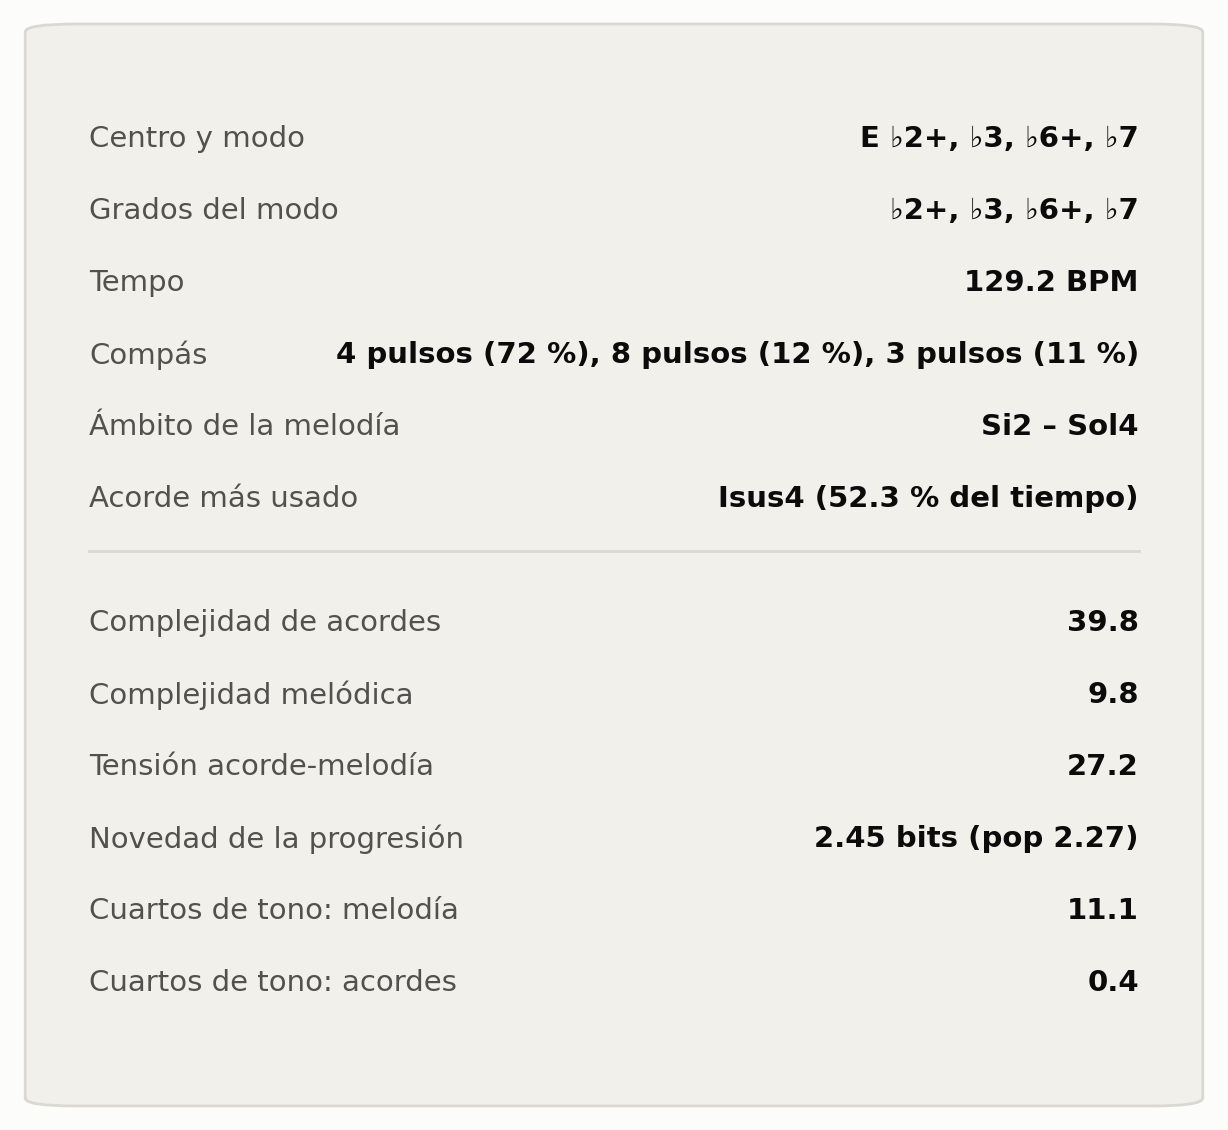
\includegraphics[width=\linewidth]{utzp_tarjeta.png}\caption{Tarjeta.}
  \end{subfigure}\hfill
  \begin{subfigure}[c]{0.55\textwidth}\centering
    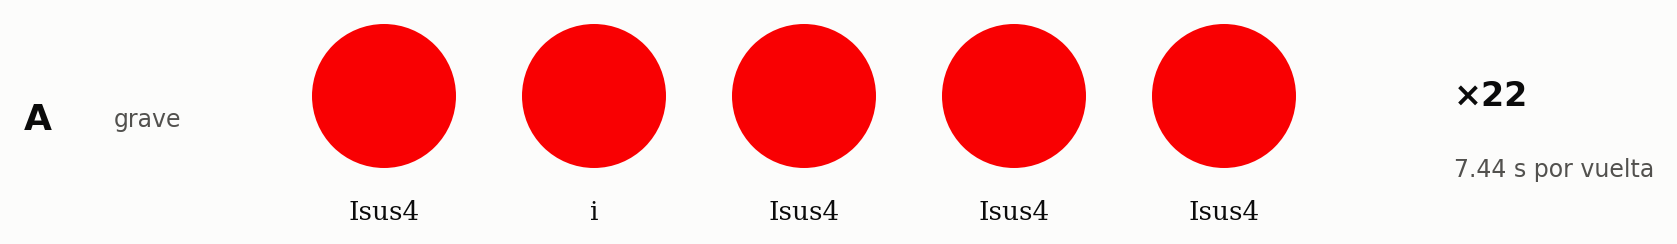
\includegraphics[width=\linewidth]{utzp_tira_de_ciclos.png}\caption{Ciclos repetidos.}
  \end{subfigure}
  \caption{Utzp: tarjeta y tira de ciclos; misma lectura que la figura~\ref{fig:fabienk-tarjeta}. Centro Mi, modo \fl2+, \fl3, \fl6+, \fl7; compases confiables: 82.2\,\%.}\label{fig:utzp-tarjeta}
\end{figure}

\begin{figure}[p]
  \centering
  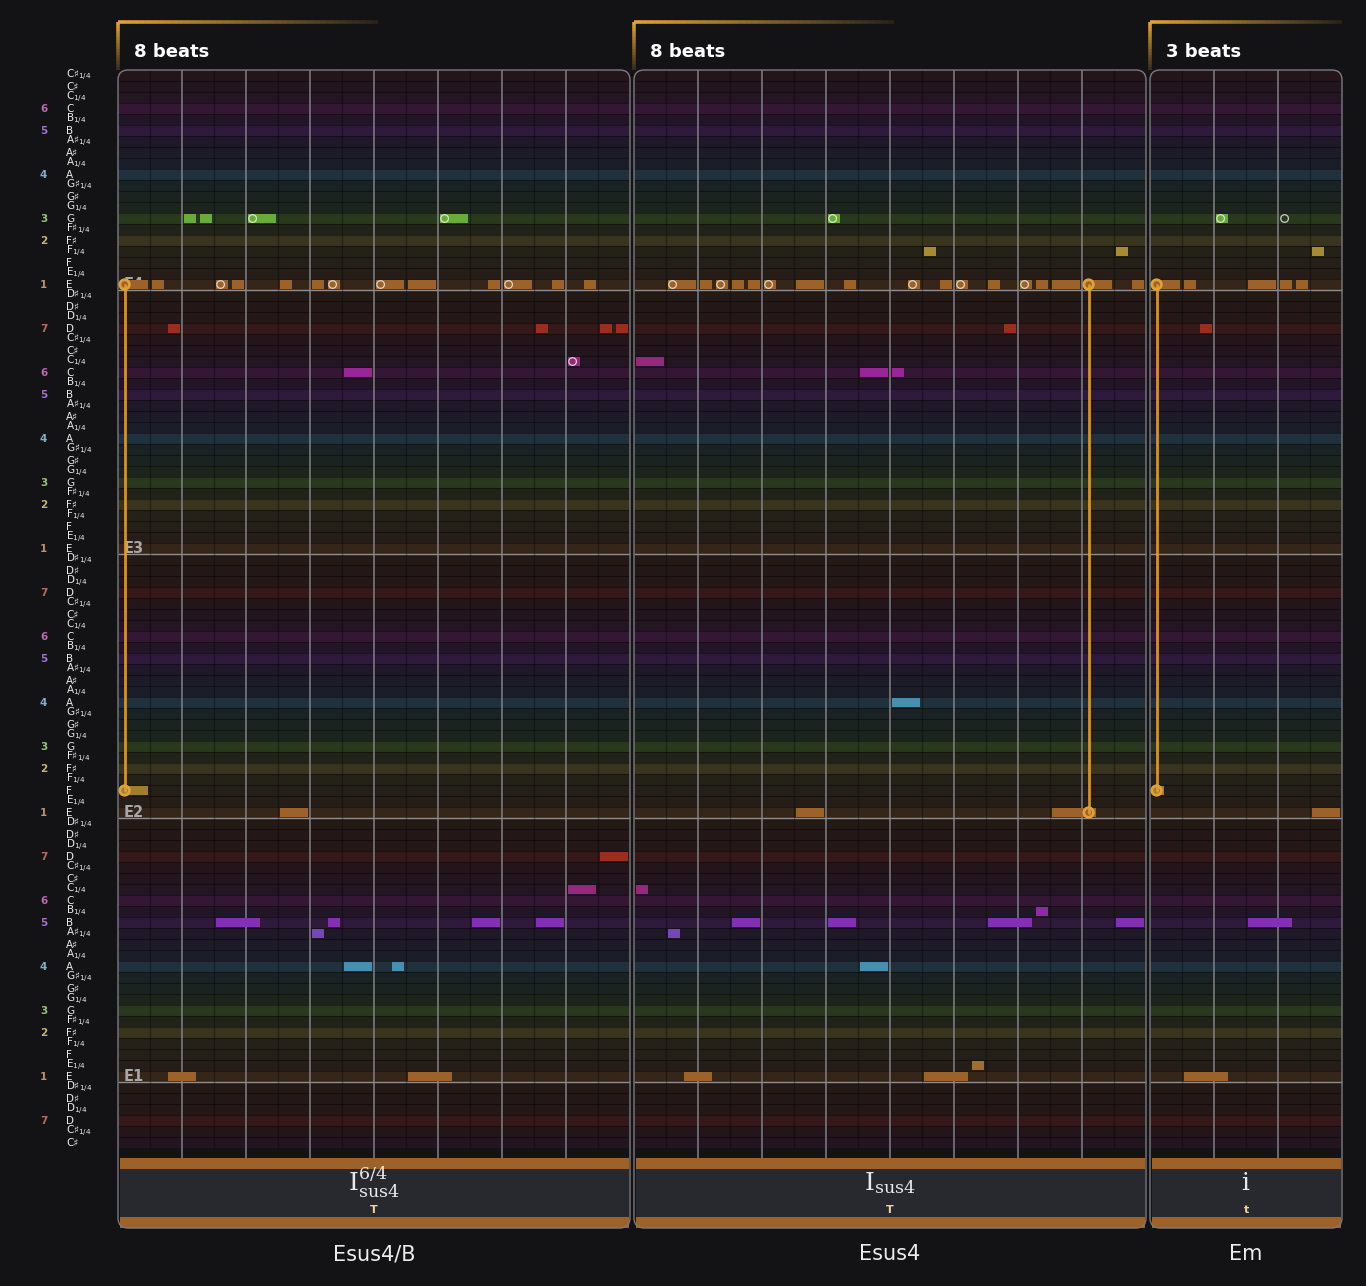
\includegraphics[width=0.75\textwidth]{utzp_tabroll24.png}\\[0.5em]
  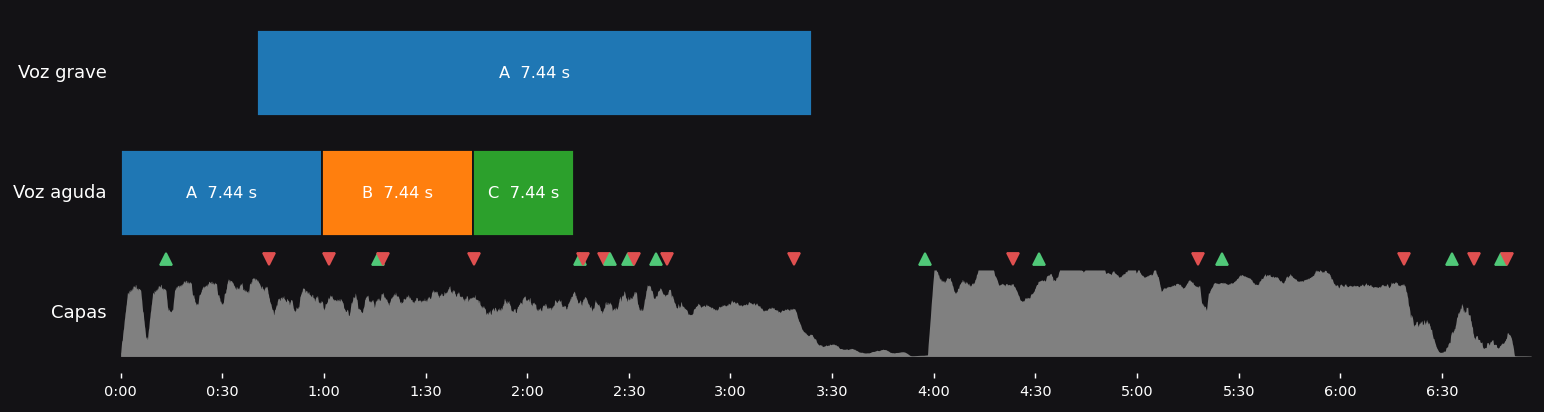
\includegraphics[width=\textwidth]{utzp_mapa_ciclos.png}
  \caption{Utzp: una página del tabroll24 (arriba) y el mapa de ciclos (abajo); misma lectura que la figura~\ref{fig:mata}.}\label{fig:utzp}
\end{figure}

\paragraph{Armonía.} Otro pedal: I el 96\,\% del tiempo (sus4 el 52\,\% y quinta sola el 31\,\%) y \fl VII el 4\,\%. De los
9 cambios, el 78\,\% son por segunda. La introducción está sobre Si (5) y entra a Mi por quinta abajo, como una cadencia de
dominante a tónica a gran escala.

\paragraph{Melodía.} La de mayor concentración: el 81.5\,\% de sus cuartos de tono cae en \fl6+ (6.0\,\%) y \fl2+ (3.0\,\%), y
\fl6+ aparece en todas las vueltas.

\paragraph{Metro y comparación.} Va en 4 (32 corcheas). Es la única canción con veredicto «síntesis de lenguajes
existentes»: en percentil por vecinos, su armonía es típica del rock (89), sus cuartos de tono del radif (32) y su metro del rock y del jazz (100),
pero ningún corpus explica la combinación.

\clearpage
\subsection{Angor}

La figura~\ref{fig:angor-tarjeta} reúne la tarjeta y la tira de ciclos; la figura~\ref{fig:angor}, una página del tabroll24 y el mapa de ciclos.

\begin{figure}[!h]
  \centering
  \begin{subfigure}[c]{0.42\textwidth}\centering
    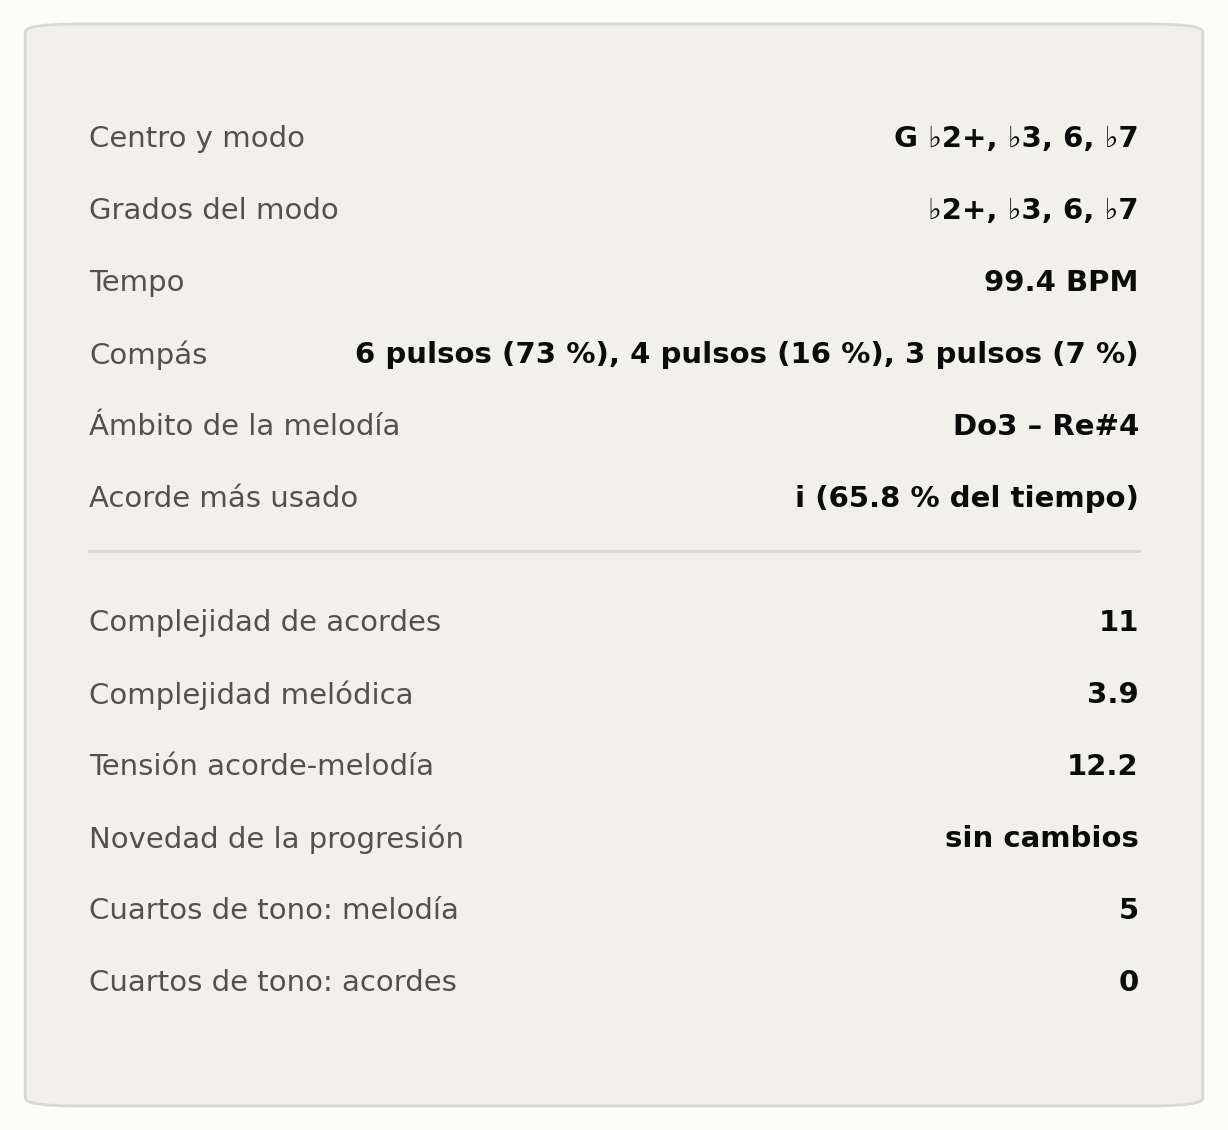
\includegraphics[width=\linewidth]{angor_tarjeta.png}\caption{Tarjeta.}
  \end{subfigure}\hfill
  \begin{subfigure}[c]{0.55\textwidth}\centering
    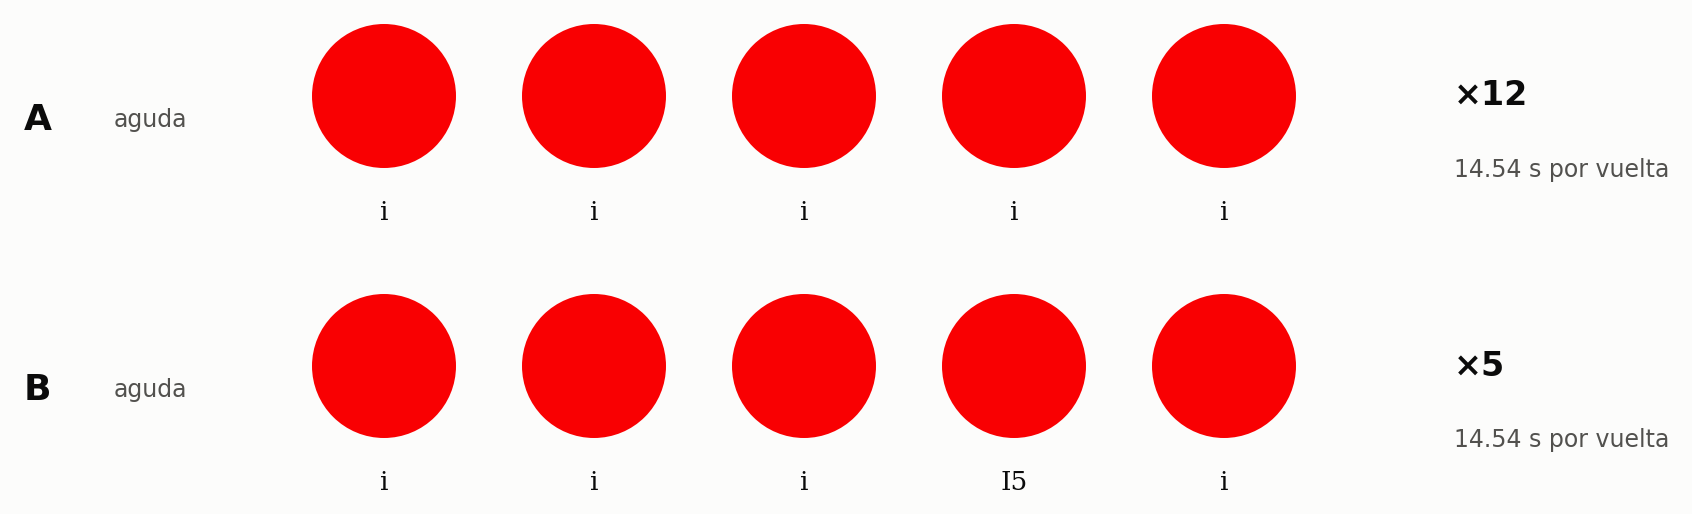
\includegraphics[width=\linewidth]{angor_tira_de_ciclos.png}\caption{Ciclos repetidos.}
  \end{subfigure}
  \caption{Angor: tarjeta y tira de ciclos; misma lectura que la figura~\ref{fig:fabienk-tarjeta}. Centro Sol, modo \fl2+, \fl3, 6, \fl7; compases confiables: 88.1\,\%.}\label{fig:angor-tarjeta}
\end{figure}

\begin{figure}[p]
  \centering
  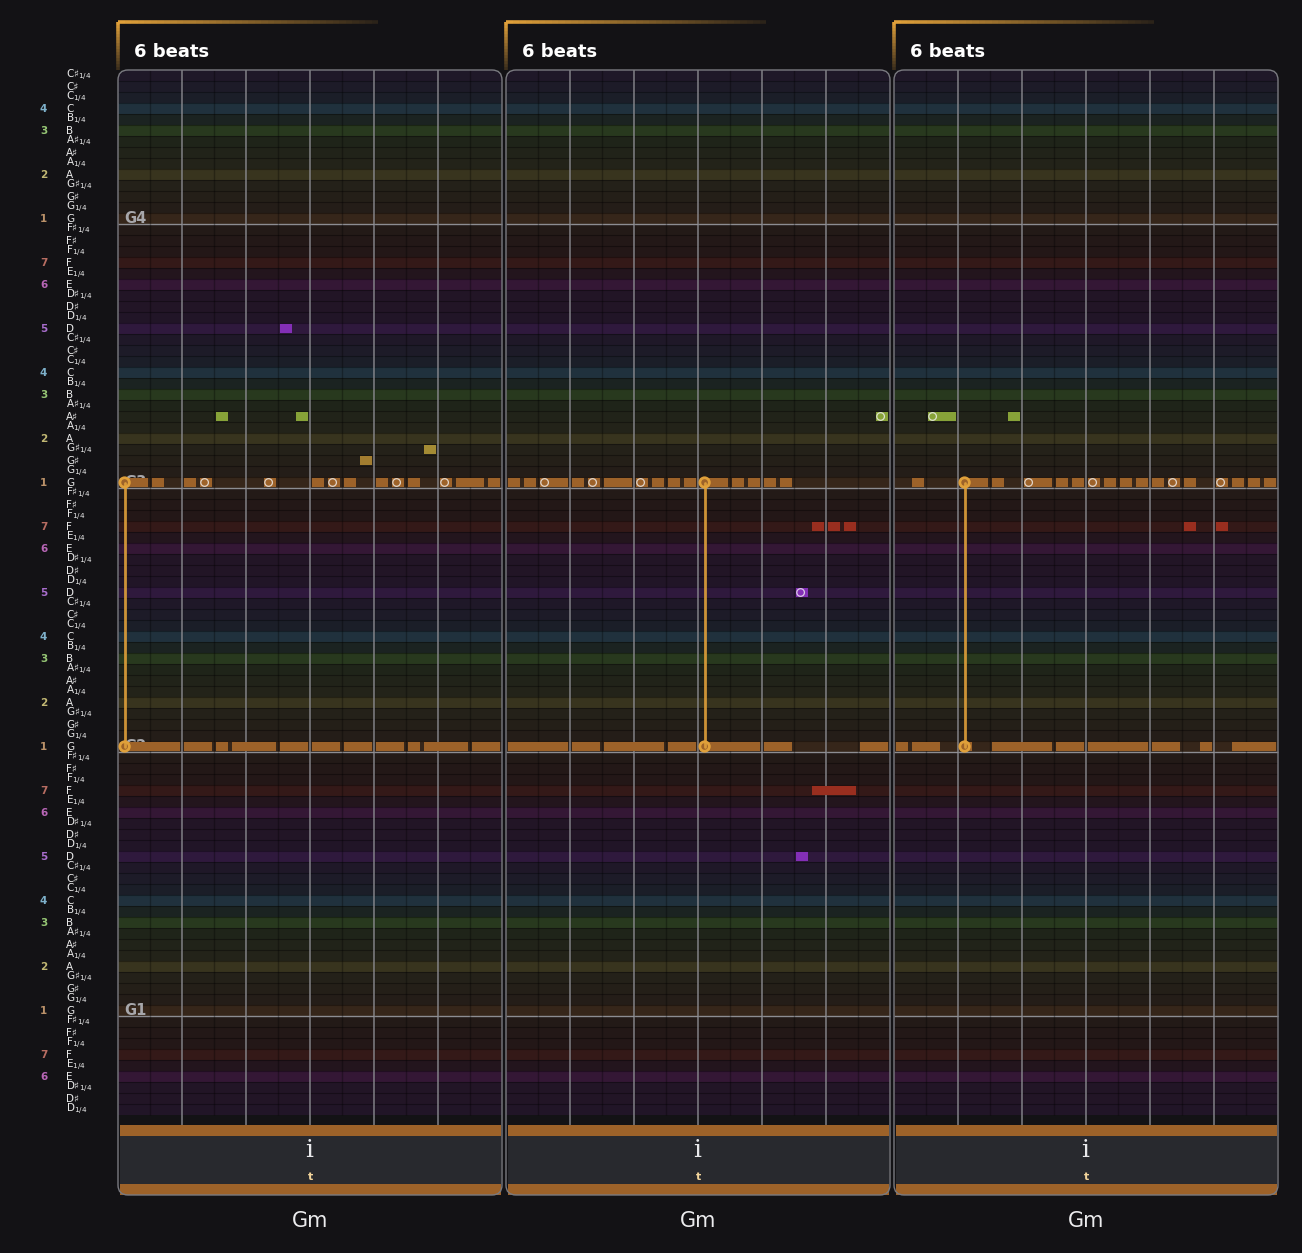
\includegraphics[width=0.75\textwidth]{angor_tabroll24.png}\\[0.5em]
  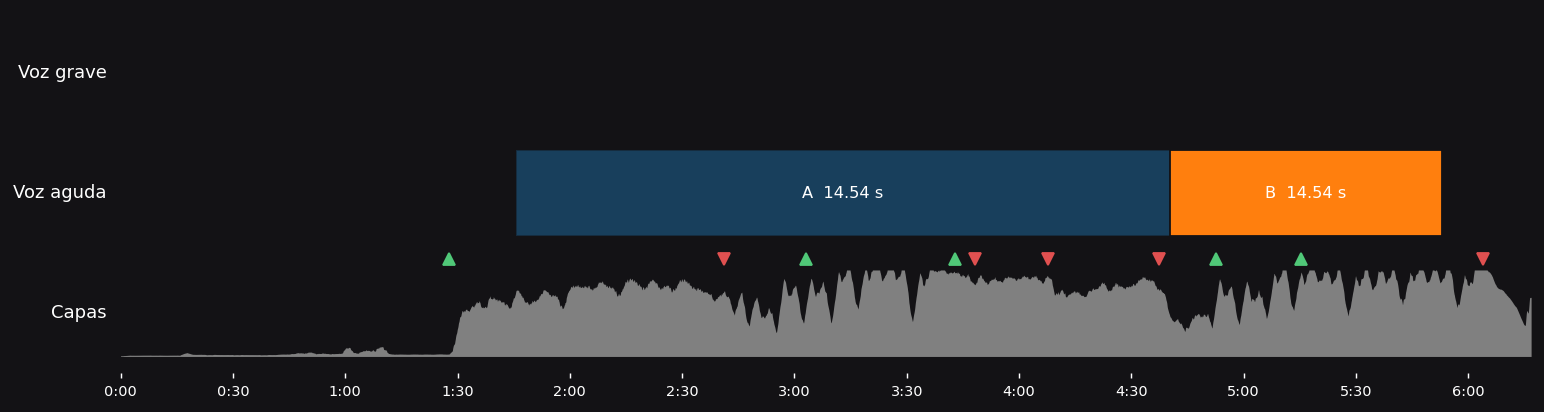
\includegraphics[width=\textwidth]{angor_mapa_ciclos.png}
  \caption{Angor: una página del tabroll24 (arriba) y el mapa de ciclos (abajo); misma lectura que la figura~\ref{fig:mata}.}\label{fig:angor}
\end{figure}

\paragraph{Armonía.} Un pedal casi absoluto: la fundamental está en I el 99.5\,\% del tiempo (i el 66\,\% y I5 el 31\,\%), sin
cambios entre compases confiables. En el test por bloques su armonía es idéntica a la de «Flying Microtonal Banana» de King
Gizzard, también un pedal sobre I.

\paragraph{Melodía.} Solo el 5\,\% de la melodía está en cuartos de tono, por debajo del piso de ruido, así que no cuenta
como evidencia. Aun así, \fl2+ aparece en el 92\,\% de las vueltas.

\paragraph{Metro.} La voz aguda repite un ciclo de 14.5~s y el mejor periodo es de 24 corcheas ($R = 0.83$); la voz grave no
tiene ciclos. Sin vecino en metro. Angor no tiene referencia de oído, así que sus cifras no se pueden evaluar.
